\documentclass[a4paper,12pt]{article}
%\usepackage{algorithm}
%\usepackage{algorithmic}
\usepackage[ruled,vlined]{algorithm2e}


% --- Encoding and Language ---
\usepackage[utf8]{inputenc}
\usepackage[T1]{fontenc}
\usepackage[english]{babel}

% --- Layout ---
\usepackage{geometry}
\geometry{a4paper, margin=1in}
\usepackage{setspace} % for \onehalfspacing

% --- Section Titles ---
\usepackage{titlesec}
\titleformat{\section}{\large\bfseries}{\thesection}{1em}{}
\titleformat{\subsection}{\normalsize\bfseries}{\thesubsection}{1em}{}

% --- Math and Graphics ---
\usepackage{amsmath, amssymb}
\usepackage{graphicx}
\usepackage{float}
\usepackage{caption}
\usepackage{subcaption}

% --- Bibliography (natbib) ---
\usepackage[numbers]{natbib} % or [authoryear]
\bibliographystyle{plainnat}

% --- Hyperlinks (load after natbib) ---
\usepackage{hyperref}
\hypersetup{
    colorlinks=true,
    linkcolor=blue,
    citecolor=blue,
    urlcolor=blue,
}

% --- Title info ---
\title{Memory-efficient PageRank on Apache Spark\\ via Random Walks}
\author{Nina Michalek \\ TU Berlin, DOS}
\date{October 28, 2025}

\begin{document}

% --- Title Page (no running headers/footers here) ---
\begin{titlepage}
\setlength{\parindent}{0pt}

% Logos row (no header package; keeps full textheight)


\vspace{8mm}

%\hrule   % <<-- draws the horizontal rule
%\vspace{10mm}

% Header text block (ragged to avoid underfull boxes)
{\raggedright
Technical University Berlin\\
Faculty IV -- Electrical Engineering and Computer Science\\
Department for Distributed and Operating Systems\par
}
\vspace{8mm}
\hrule   % <<-- draws the horizontal rule
\vspace{10mm}

\vspace{15mm}

\begin{center}
\Large Bachelor Thesis\\[15mm]
\Huge \textbf{Memory-efficient PageRank on Apache Spark\\ via Random Walks}
\end{center}

\vspace{10mm}

% Centered "submitted by" block
\begin{center}
\begin{tabular}{rl}
submitted by: & Nina Michalek \\
Matrikel-Nr.: & 469109 \\
\end{tabular}
\end{center}

\vspace{8mm}

\begin{center}
\onehalfspacing
for obtaining the academic degree \\
\large \textbf{Bachelor of Science} \\
\normalsize (B.\,Sc.)
\end{center}

\vfill

% Bottom info block
\onehalfspacing
\begin{tabular}{@{}ll}
First examiner: & Prof.\ Dr.\ habil.\ Odej Kao\\
Second examiner: & Prof. \ Dr. \ Markl \\
Advisor: & Jonathan Will\\
Date of submission: & \today
\end{tabular}

\end{titlepage}
% --- End Title Page ---

% --- TOC + Main Document ---
\tableofcontents
\newpage

\section*{Abstract}

Standard iterative PageRank implementations encounter significant memory challenges for large-scale graph analysis as they require to store the entire graph structure, which takes up $O(n^2)$ space. Therefore iterative methods are not able to successfully operate on graphs with millions of nodes in memory constraint environments.\par

This thesis addresses this problem by proposing Monte Carlo PageRank, an approximate PageRank algorithm that estimates ranks via random walk simulation. At the beginning a fixed number of walkers per node is initialized that traverse the graph according to the random surfer model. The ranks are then estimated by the visiting frequency of each node. This approachs memory consumption is only controlled by the number of walkers rather than the graph size. The method is implemented in Apache Spark based on RDDs for distributed processing.\par

Experiments on real world and synthetic Erdős–Rényi graphs with up to 20 million nodes demonstrate that Monte Carlo PageRank is able to successfully operate with only 450 MiB across all graph sizes while GraphX standard PageRank method requires 2-8 GiB on the same datasets. Under memory constraint conditions Monte Carlo PageRank maintains stable runtimes while GraphX either fails or encounters performance issues. The approximate method achieves 75\% to 90\% accuracy on the top 20 nodes depending on the walker count on 5-10 times lower resource costs measured in GiB-hours compared to standard iterative PageRank. \par

Monte Carlo PageRank demonstrates a memory efficient alternative for large scale graph analytics under memory constraint conditions where standard methods fail to operate while achieving an acceptable accuracy.







\newpage
\section{Introduction}
Graphs are widely used to represent relationships between different entities for applications such as social networks and website links \cite{zhang_distributed_2021}. 
A wide range of graph algorithms have been developed to analyse these structures. \cite{malewicz_pregel_2010}\cite{low_distributed_2012}\cite{koch_empirical_2016}. Among the most influential is PageRank \cite{page_pagerank_1999}, an iterative algorithm introduced by Google to determine the importance of websites. Faced with the challenge of information retrieval posed by the rapid expansion of the World Wide Web in the late 1990s, PageRank provided a method of ranking web pages by measuring their relative importance based on the graph of the web. In this graph, the nodes are the web pages, while the edges represent links. An outedge is a link on a page and an inedge is a backlink. The core idea is that a page is considered important if it has inedges from important pages.\par
The PageRank value of a web page is calculated iteratively based on the values of all the pages that link to it. Linking pages pass on a fraction of their own value, proportional to their number of outbound links, to the target page. This calculation includes a damping factor that converges to a stable probability distribution, effectively representing the probability that a random user will end up on a particular page.
Today, PageRank is used not only in search engines, but in a wide range of applications such as social networks \cite{wu_efficient_2024}. These networks use PageRank to identify influential users, rank content in feeds and recommend people \cite{weng_twitterrank_2010}.\par
Despite its wide applicability, a fundamental challenge lies in the representation of graphs \cite{liu_fast_2015}. Typically, graphs are represented in matrices, which in the worst case require up to $O(n^2)$ of memory, where $n$ is the number of web pages \cite{wu_efficient_2024}. The transition matrix, which contains the probabilities of moving from one web page to another in a single step, presents a significant memory challenge as graph sizes grow.\par
To meet the demands of graph analytics, specialised graph processing frameworks have been introduced. These systems are designed to efficiently execute iterative algorithms, making graph analytics more practical. An example of such a system is GraphX \cite{xin_graphx_2013}, which is based on Apache Spark \cite{xin_graphx_2013}, a popular open source distributed dataflow system that enables large-scale data processing \cite{shanahan_large_2015}. GraphX acts as a graph processing framework that aims to bridge the gap between system-level optimisations in specialised graph engines and the flexible dataflow operations available in general-purpose systems \cite{jin_software_2022}. However, even with such frameworks, the memory consumption of algorithms such as PageRank can be enormous. Therefore, recent research has attempted to address the memory overhead in GraphX's PageRank algorithm due to the data representation, and proposes approximate computation to reduce memory consumption \cite{wu_efficient_2024}. 
\newpage

\section{Background and Related Work}
\subsection{The PageRank Algorithm}
% Describe how PageRank works: power iteration, damping factor, convergence.

% \subsubsection{Origins and Motivation}
% \subsubsection{Graph Representation and the Transition Matrix}
% \subsubsection{The Random Surfer Model and Damping Factor}
% \subsubsection{Mathematical Definition of PageRank}
% \subsubsection{Power Iteration and Convergence}
% \subsubsection{Complexity and other Variants (Personalized PageRank)}


PageRank is an algorithm that was originally introduced to measure the relevance of websites on the World Wide Web. The more websites that link to a website, the higher its rank. Created by Google founders Larry Page and Sergey Brin, it was designed to optimize the search engine \cite{page_pagerank_1999}.
The algorithm is based on a graph where each node represents a website on the internet, and each edge represents a hyperlink on a website.
\begin{figure}[ht]
    \centering
    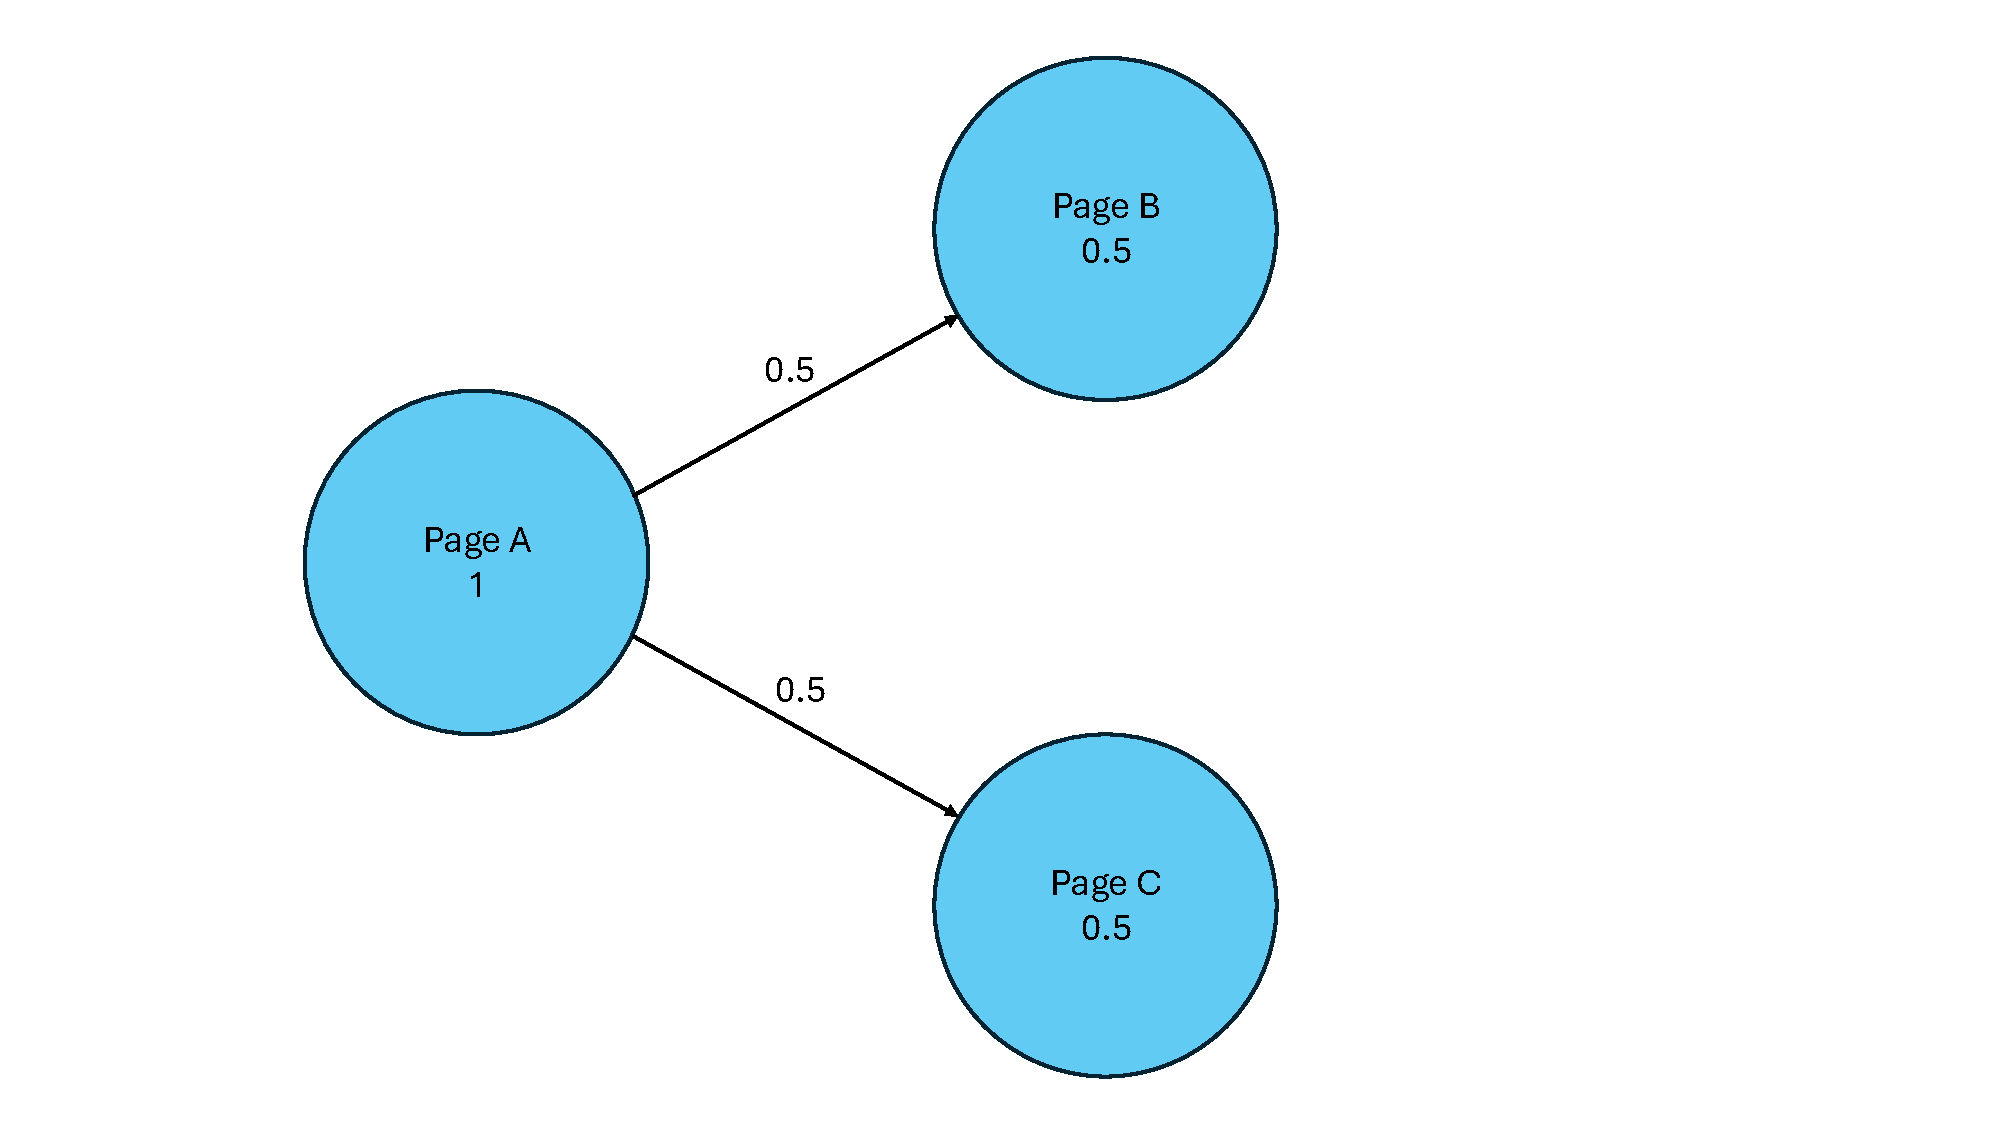
\includegraphics[width=0.7\linewidth]{images/PageRank_Graph.pdf}
    \caption{PageRank Propagation along Edges}
    \label{fig:pagerank}
\end{figure}
\begin{figure}[ht]
    \centering
    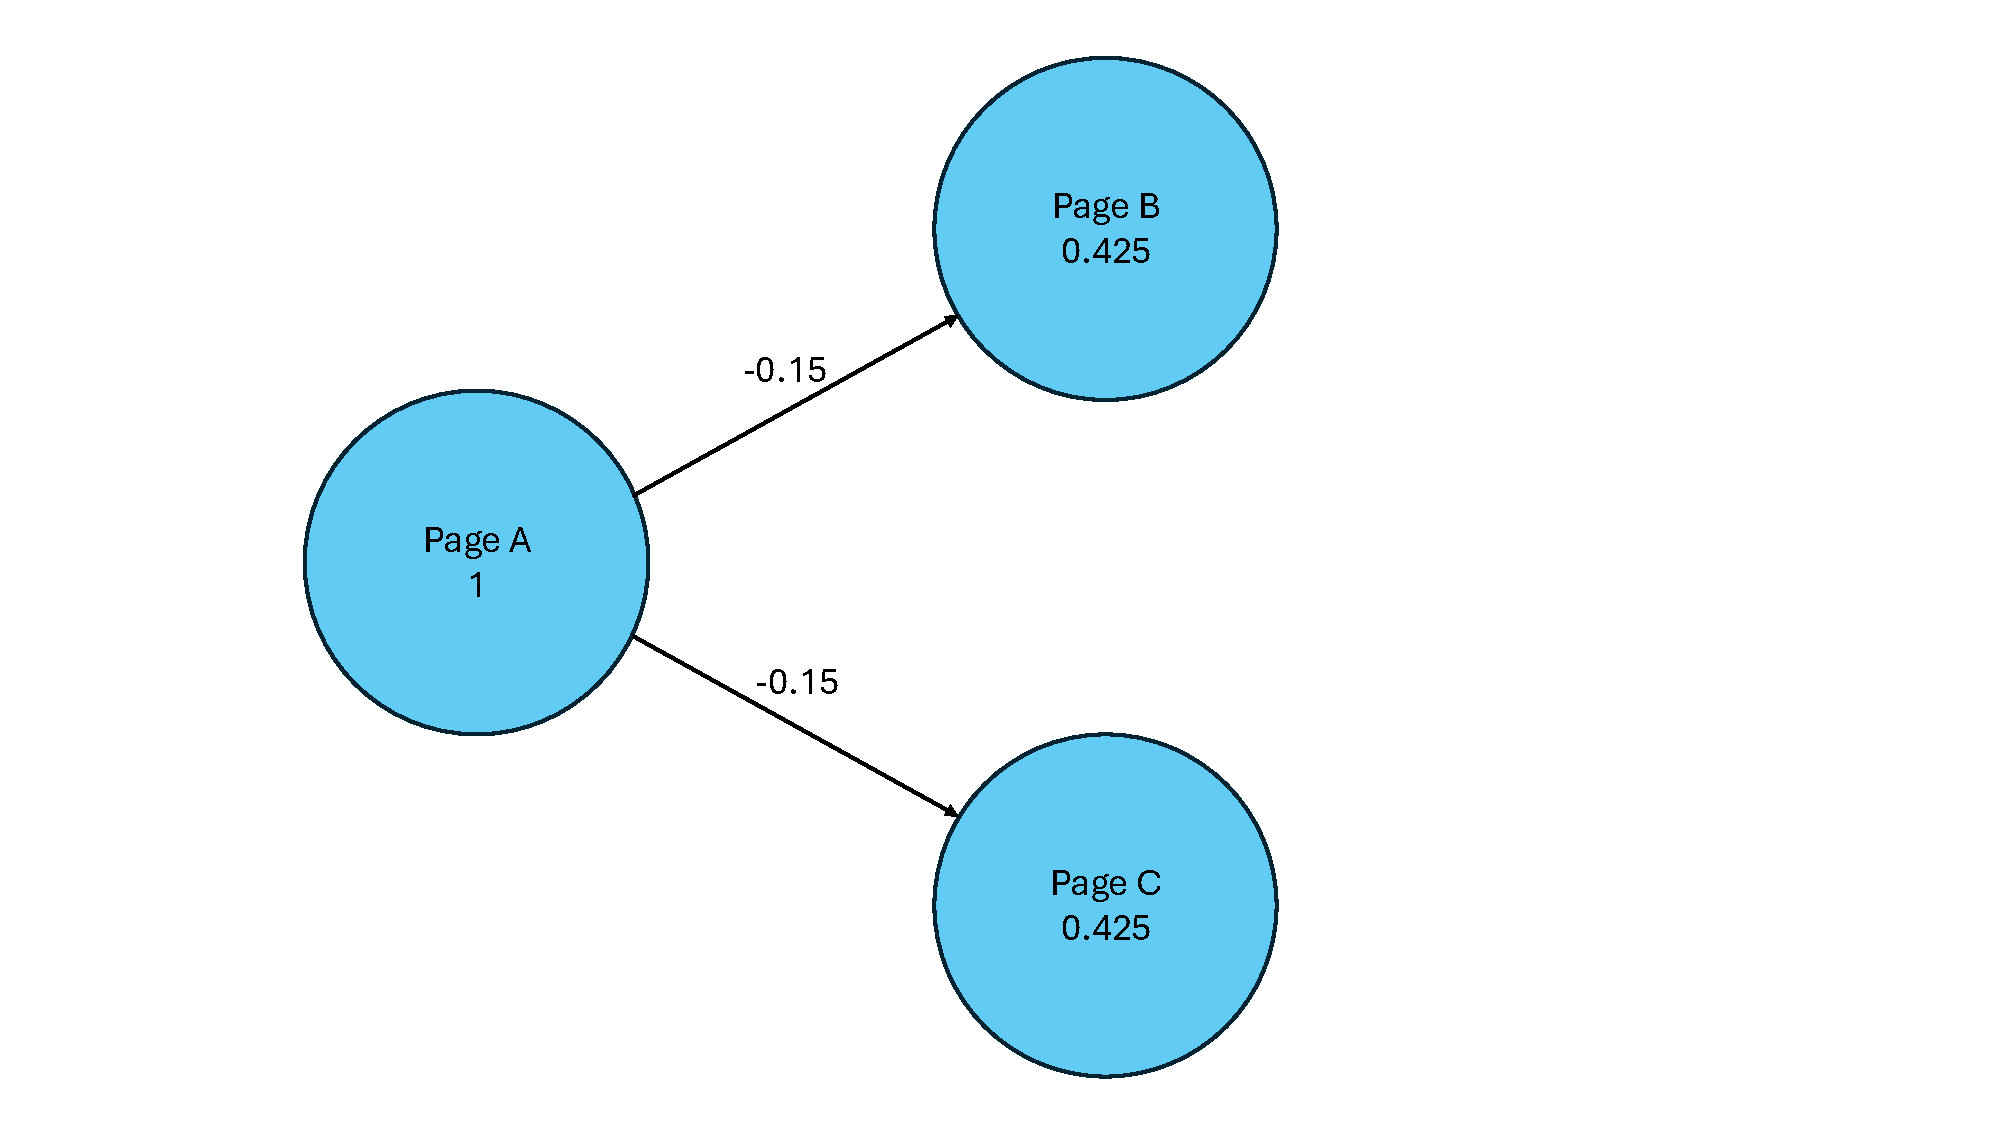
\includegraphics[width=0.7\linewidth]{images/PageRank_Graph_DF.pdf}
    \caption{PageRank Propagation with Damping Factor}
    \label{fig:pagerankdf}
\end{figure}

% \begin{figure}[H]
%     \centering
%     \begin{subfigure}[t]{0.7\linewidth}
%         \centering
%         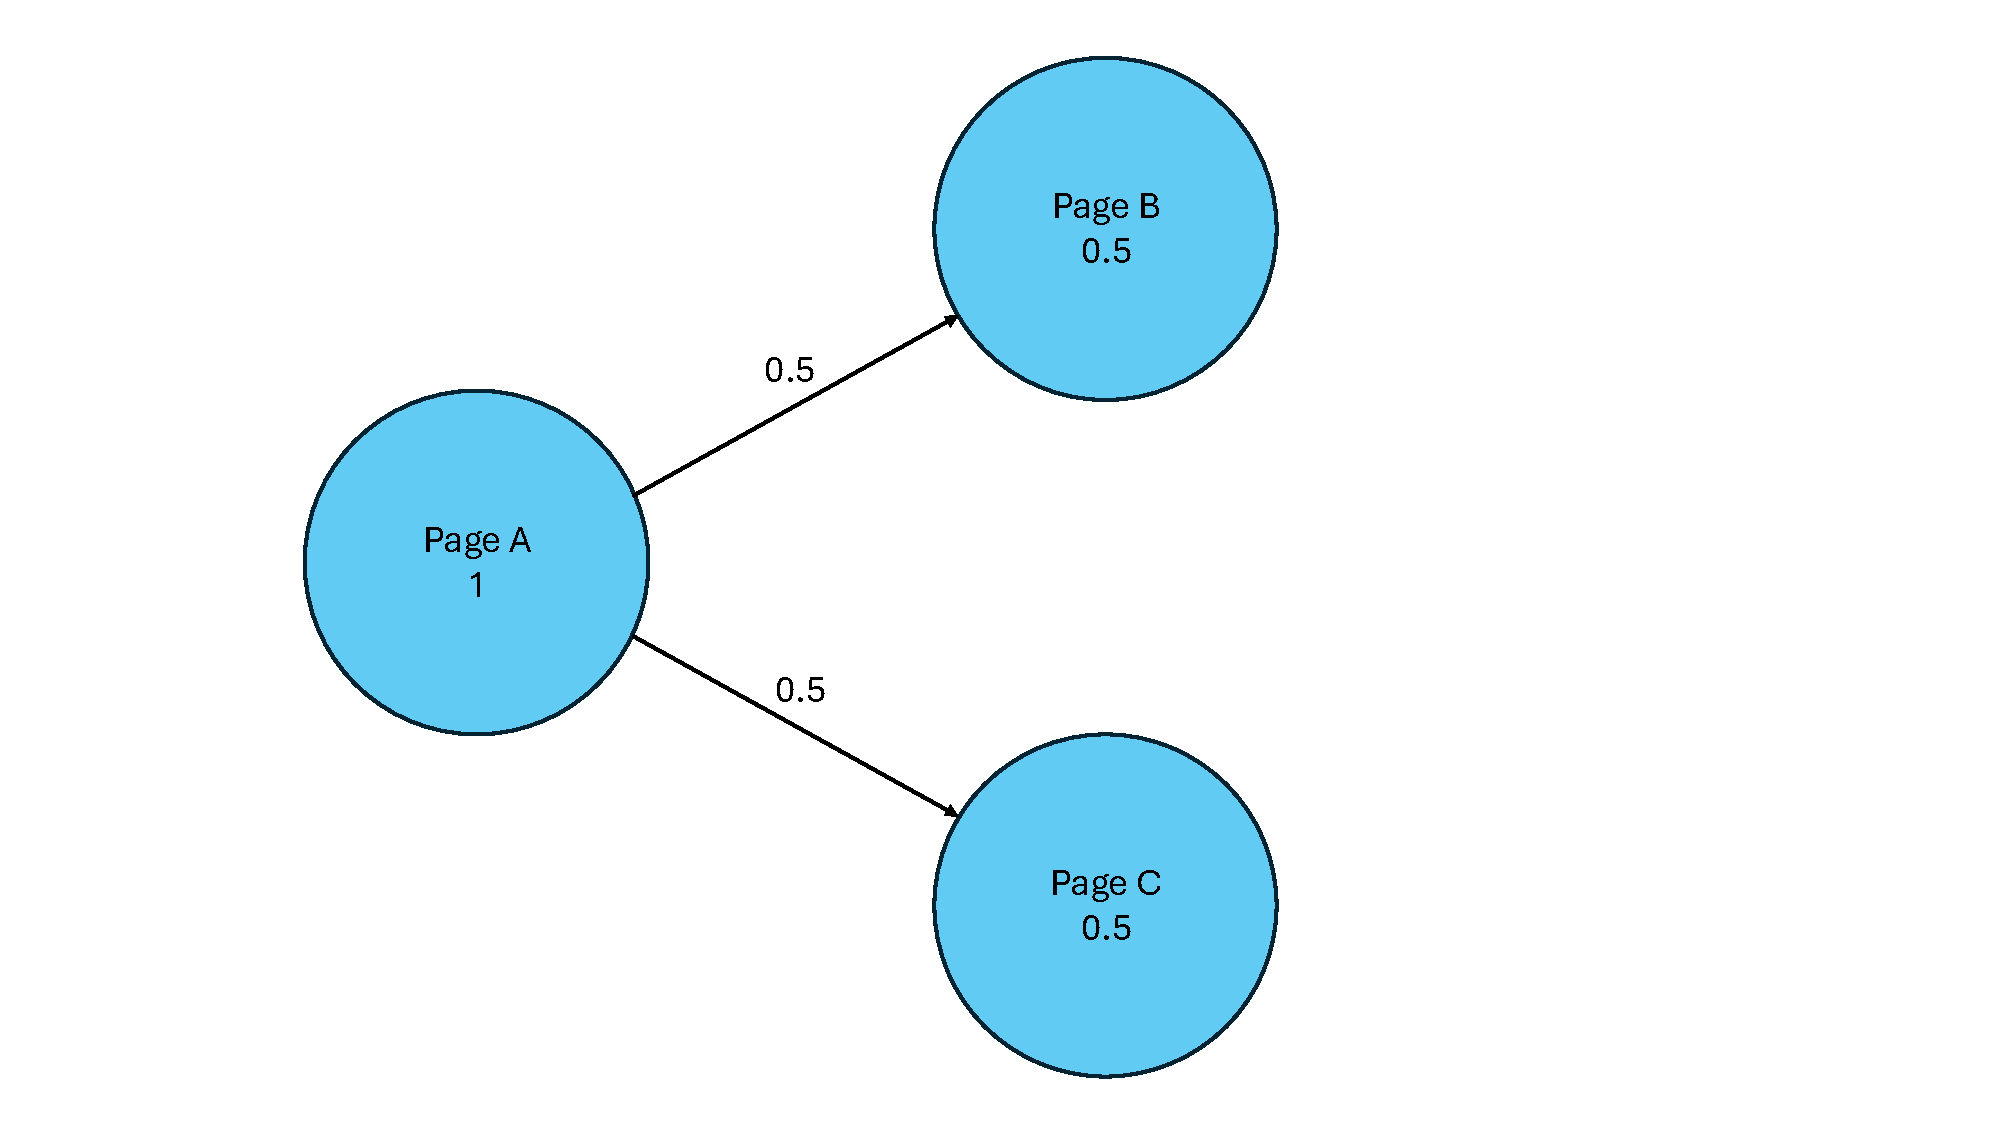
\includegraphics[width=\linewidth]{images/PageRank_Graph.pdf}
%         \caption{2 edges per node}
%         \label{fig:2run}
%     \end{subfigure}\hfill
%     \begin{subfigure}[t]{0.7\linewidth}
%         \centering
%         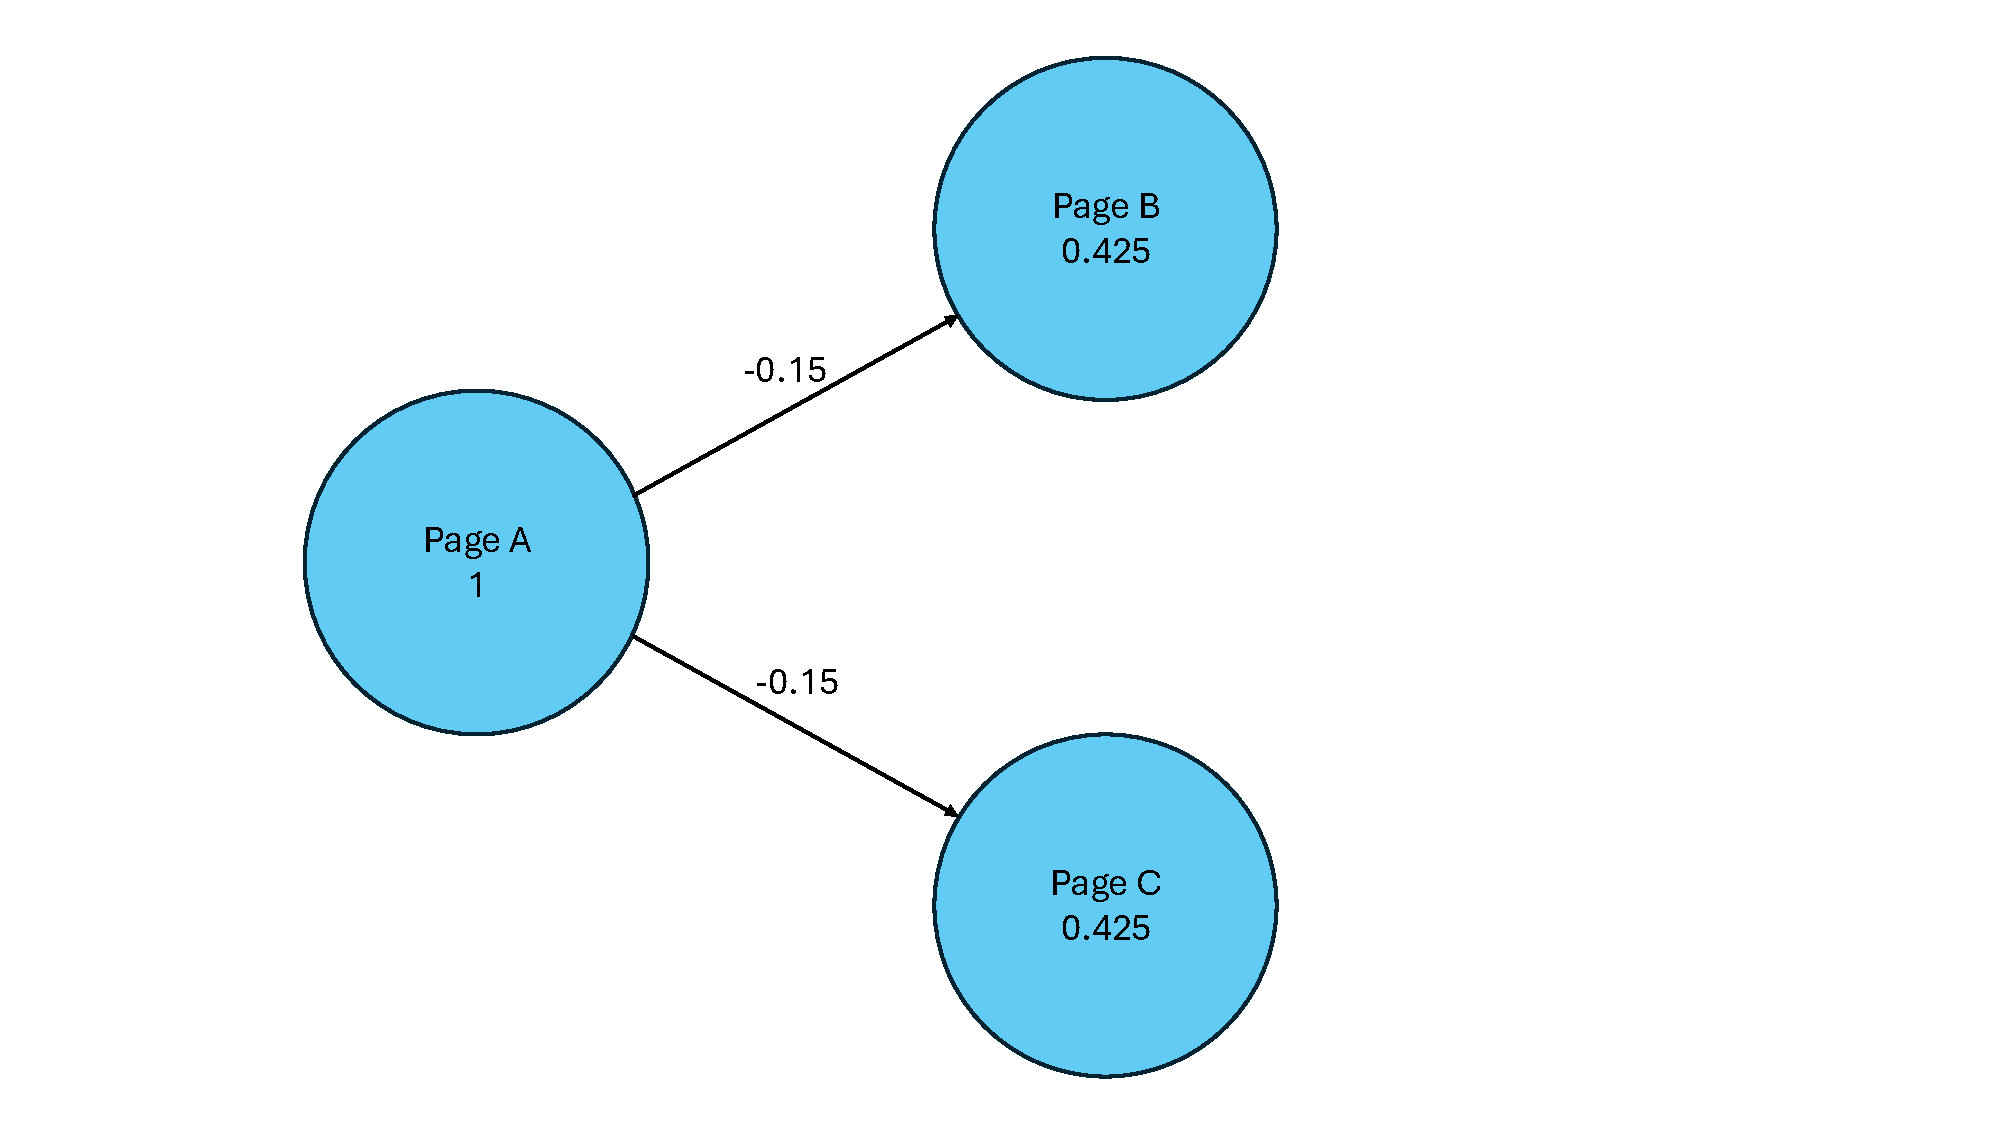
\includegraphics[width=\linewidth]{images/PageRank_Graph_DF.pdf}
%         \caption{2 edges per node}
%         \label{fig:2cost}
%     \end{subfigure}
% \end{figure}

To calculate PageRank values, a transition matrix is constructed. Each row of the matrix represents a state or website and contains the probabilities of moving from one node to another. Figure 1 shows that A has two outgoing edges, so the probability of moving from D to another node is $0.5$. The transition matrix describes the behavior of a "random surfer". The random surfer model describes the probability of a random user visiting a website. Finding the PageRank values is a Markov chain process, and its stationary distribution is the PageRank vector. Additionally, to model realistic user behavior, a damping factor is introduced, which is commonly set to 0.85. That means with probability $\alpha$, a random surfer clicks on an outgoing hyperlink on the current website and with probability $1-\alpha$ the surfer "teleports" to a random website in the graph. This characteristic is necessary for PageRank because web graphs may contain dangling nodes, disconnected parts, or cycles. Thus, the damping factor ensures that the Markov chain is irreducible and aperiodic, guaranteeing convergence to a unique stationary distribution \cite{langville_googles_2012}. 
The PageRank algorithm is commonly defined as follows \cite{chebolu_pagerank_2008}:
\begin{equation}
    \pi_v = \frac{1-\alpha}{n}+c\sum_{u\in N^-(v)}\frac{\pi_u}{d^+(u)} 
\end{equation} 
where: 
\begin{itemize}
    \item $\pi_v$ is the PageRank of the node $v$
    \item $\alpha$ is the damping factor
    \item $n$ is the total number of nodes in the graph
    \item $N^-(v)$ is the set of ingoing edges of $v$
    \item $d^+(u)$ is the out degree of $u$
\end{itemize} 
% talk about tolerance and convergence
The calculation of PageRank follows the power iteration method, a technique to finding the dominant eigenvalue. The iterative process is defined as follows
\begin{enumerate}
    \item Define the initial vector 
    \begin{equation}
        \pi^{(0)}=\frac{1}{n}e
    \end{equation}
    \item At each iteration apply the update rule, where $S$ is the transition matrix and $e$ is the all-ones vector
    \begin{equation}
        \pi^{(k+1)} = \alpha S^T+ \frac{(1-\alpha)}{n}e
    \end{equation}
    \item Continue until the difference between iterations is less than a tolerance $\epsilon$
    \begin{equation}
        ||\pi^{(k+1)}-\pi^{(k)}||_1<\epsilon \quad \text{\cite{langville_googles_2012}\cite{page_pagerank_1999}}
    \end{equation}
    
\end{enumerate}
Then $\pi$ satisfies 
\begin{equation}
    \pi=G^T\pi, \quad \text{where $G=\alpha S +\frac{1-\alpha}{n}ee^T$}
\end{equation}
and $\pi$ is a stationary probability distribution, the unique PageRank vector.
Each entry in the PageRank vector represents the probability that a random surfer will land on a particular node. The power iteration method has a time complexity of $O(m)$ per iteration, where $m$ is the the number of edges. Thus, the total complexity is $O(m\cdot k)$. The number of iterations, $k$, depends on the damping factor, $\alpha$, and the tolerance ,$\epsilon$. After the original PageRank algorithm was introduced, many more variants were developed, such as Personalized PageRank (PPR) \cite{park_survey_2019}.
In this version, teleportation is not uniformly distributed across all nodes. Instead, the random surfer only jumps to a specific set of nodes called  "restarting nodes". The resulting PageRank vector measures how close or relevant each node is to the restarting nodes in the set \cite{priyanta_social_2019}. 

 
% \subsection{Challenges in Large-Scale Graph Processing}

% \subsubsection{Growth of Graph Data}
% \subsubsection{Memory Bottlenecks of PageRank}
% \subsubsection{Computational Complexity and Iterations}
% \subsubsection{Limits of Single-Machine Processing}
% \subsubsection{Distributed Graph Processing Challenges}

% Memory and computational bottlenecks with big graphs
When PageRank was introduced, there were already about 150 million websites. Today, even larger amounts of graph data are generated by applications such as social networks and communication networks \cite{gebreegziabher_chapter_2023}. Thus, analyzing these large-scale graphs has become a significant challenge due to memory limitations. The PageRank algorithm requires storing the entire transition matrix, which takes up to $O(n^2)$ space in the worst case. Therefore, it is not feasible for large graphs with a billion nodes \cite{wu_efficient_2024}. Each iteration requires the entire graph structure to be stored in memory, and it can take around a hundred iterations to converge \cite{langville_googles_2012}, with a cost of $O(m)$ per iteration, creating a significant computational overhead. Often, a single machine is insufficient for large-scale graph analytics tasks due to memory and computing power limitations. On the other hand, applying large graphs to distributed systems presents numerous challenges, such as parallelism and load balancing. To address these challenges, many distributed graph systems have been proposed to store large graphs on multiple machines and compute algorithms like PageRank, including Pregel \cite{meng_survey_2024}.



% \subsection{Apache Spark and GraphX}
% % Explain architecture, vertex-centric computation, and limits of GraphX PageRank.

% % \subsubsection{Pregel and Vertex-Centric Computation}
% % \subsubsection{Integration of GraphX into Spark}
% % \subsubsection{Optimizations in GraphX (Partitioning, Joins)}
% % \subsubsection{Strengths and Flexibility of GraphX}
% % \subsubsection{Limitations for Very Large Graphs}

% GraphX is a library built on top of Apache Spark that specializes in large graph processing. It provides a powerful Pregel API that can implement the specialized graph parallel system abstraction described in\cite{malewicz_pregel_2010} and a simple representation of data in relational algebra described in \cite{xin_graphx_2014}. Pregel is a specialized graph processing system originally introduced by Google \cite{malewicz_pregel_2010}. It uses a vertex centric technique that follows the philosophy of "think like a vertex", where a graph analytics algorithm iteratively executes a program over vertices \cite{xin_graphx_2014}. 
% Specialized systems like Pregel are optimized for graph algorithms, but they are not suitable for practical use since they lack the flexibility to combine graph analysis with broader data processing tasks and the integration of such systems with other data stacks is limited. In contrast, GraphX's integration into Spark's unified analytics platform allows for the seamless combination of graph analytics and other data pipelines. This approach eliminates the need for external ETL integration and data movement, both of which are common with specialized systems. Additionally, GraphX offers optimizations such as vertex-cut partitioning and join elimination, positively impacting communication and runtime \cite{xin_graphx_2014}. Nevertheless, GraphX suffers from the general-purpose nature of the Apache Spark system and may struggle with runtime and very large graphs due to its high memory demand \cite{zhuo_distributed_2021}.  
% Finally, GraphX achieves comparable performance to systems like Pregel, while also providing an efficient, end-to-end analytics pipeline. This makes GraphX a more versatile framework for real-world applications \cite{xin_graphx_2014}.

\subsection{Apache Spark and GraphX}
GraphX is a library built on top of Apache Spark that specializes in large graph processing. It provides a powerful Pregel API that can implement the specialized graph parallel system abstraction described in\cite{malewicz_pregel_2010} and a simple representation of data in relational algebra described in \cite{xin_graphx_2014}. Pregel is a specialized graph processing system originally introduced by Google \cite{malewicz_pregel_2010}. It uses a vertex centric technique that follows the philosophy of "think like a vertex", where a graph analytics algorithm iteratively executes a program over vertices \cite{xin_graphx_2014}. \par

A Resilient Distributed Dataset (RDD) is the core abstraction in Spark. An RDD is a partitioned collection of elements that is distributed across the nodes of a cluster. It is processed in parallel \cite{apache_spark_rdd_2025}. RDDs are immutable and resilient to failures due to lineage, which is a feature that records all transformations applied to the data. In the event of a node failure, lost data can be recomputed using these records. RDDs can perform two types of operations: transformations and actions. Each transformation, such as map, filter, or join, creates a new RDD. An action, such as count, triggers execution. RDDs can be cached or persisted in memory to avoid recomputation with each iteration \cite{chambers_spark_2018}. However, since RDDs are immutable, every transformation creates a new RDD. This can easily result in high memory usage, especially when computing iterative graph algorithms, such as PageRank, where each iteration creates new RDDs for vertex properties. \par

Specialized systems like Pregel are optimized for graph algorithms, but they are not suitable for practical use since they lack the flexibility to combine graph analysis with broader data processing tasks and the integration of such systems with other data stacks is limited. In contrast, GraphX's integration into Spark's unified analytics platform allows for the seamless combination of graph analytics and other data pipelines. This approach eliminates the need for external ETL integration and data movement, both of which are common with specialized systems. Additionally, GraphX offers optimizations such as vertex-cut partitioning and join elimination, positively impacting communication and runtime \cite{xin_graphx_2014}. Nevertheless, GraphX suffers from the general-purpose nature of the Apache Spark system and may struggle with runtime and very large graphs due to its high memory demand \cite{zhuo_distributed_2021}.  \par
Finally, GraphX achieves comparable performance to systems like Pregel, while also providing an efficient, end-to-end analytics pipeline. This makes GraphX a more versatile framework for real-world applications \cite{xin_graphx_2014}.


\subsection{Spark's Memory Management}

% \subsubsection{Executor Memory and JVM Heap Space}
% \subsubsection{Reserved Memory}
% \subsubsection{Unified Memory: Spark vs. User Memory}
% \subsubsection{Execution vs. Storage Memory}
% \subsubsection{Dynamic Occupancy Mechanism}
% \subsubsection{On-Heap vs. Off-Heap Memory}

The memory allocation in Apache Spark is crucial for the performance of Spark applications. Spark uses a unified memory called the JVM Heap Space, also known as the Spark Executor Heap Space. The amount of JVM heap memory allocated to each executor is referred to as spark.executor.memory. This memory is then distributed into three parts: 

\begin{figure}[ht]
    \centering
    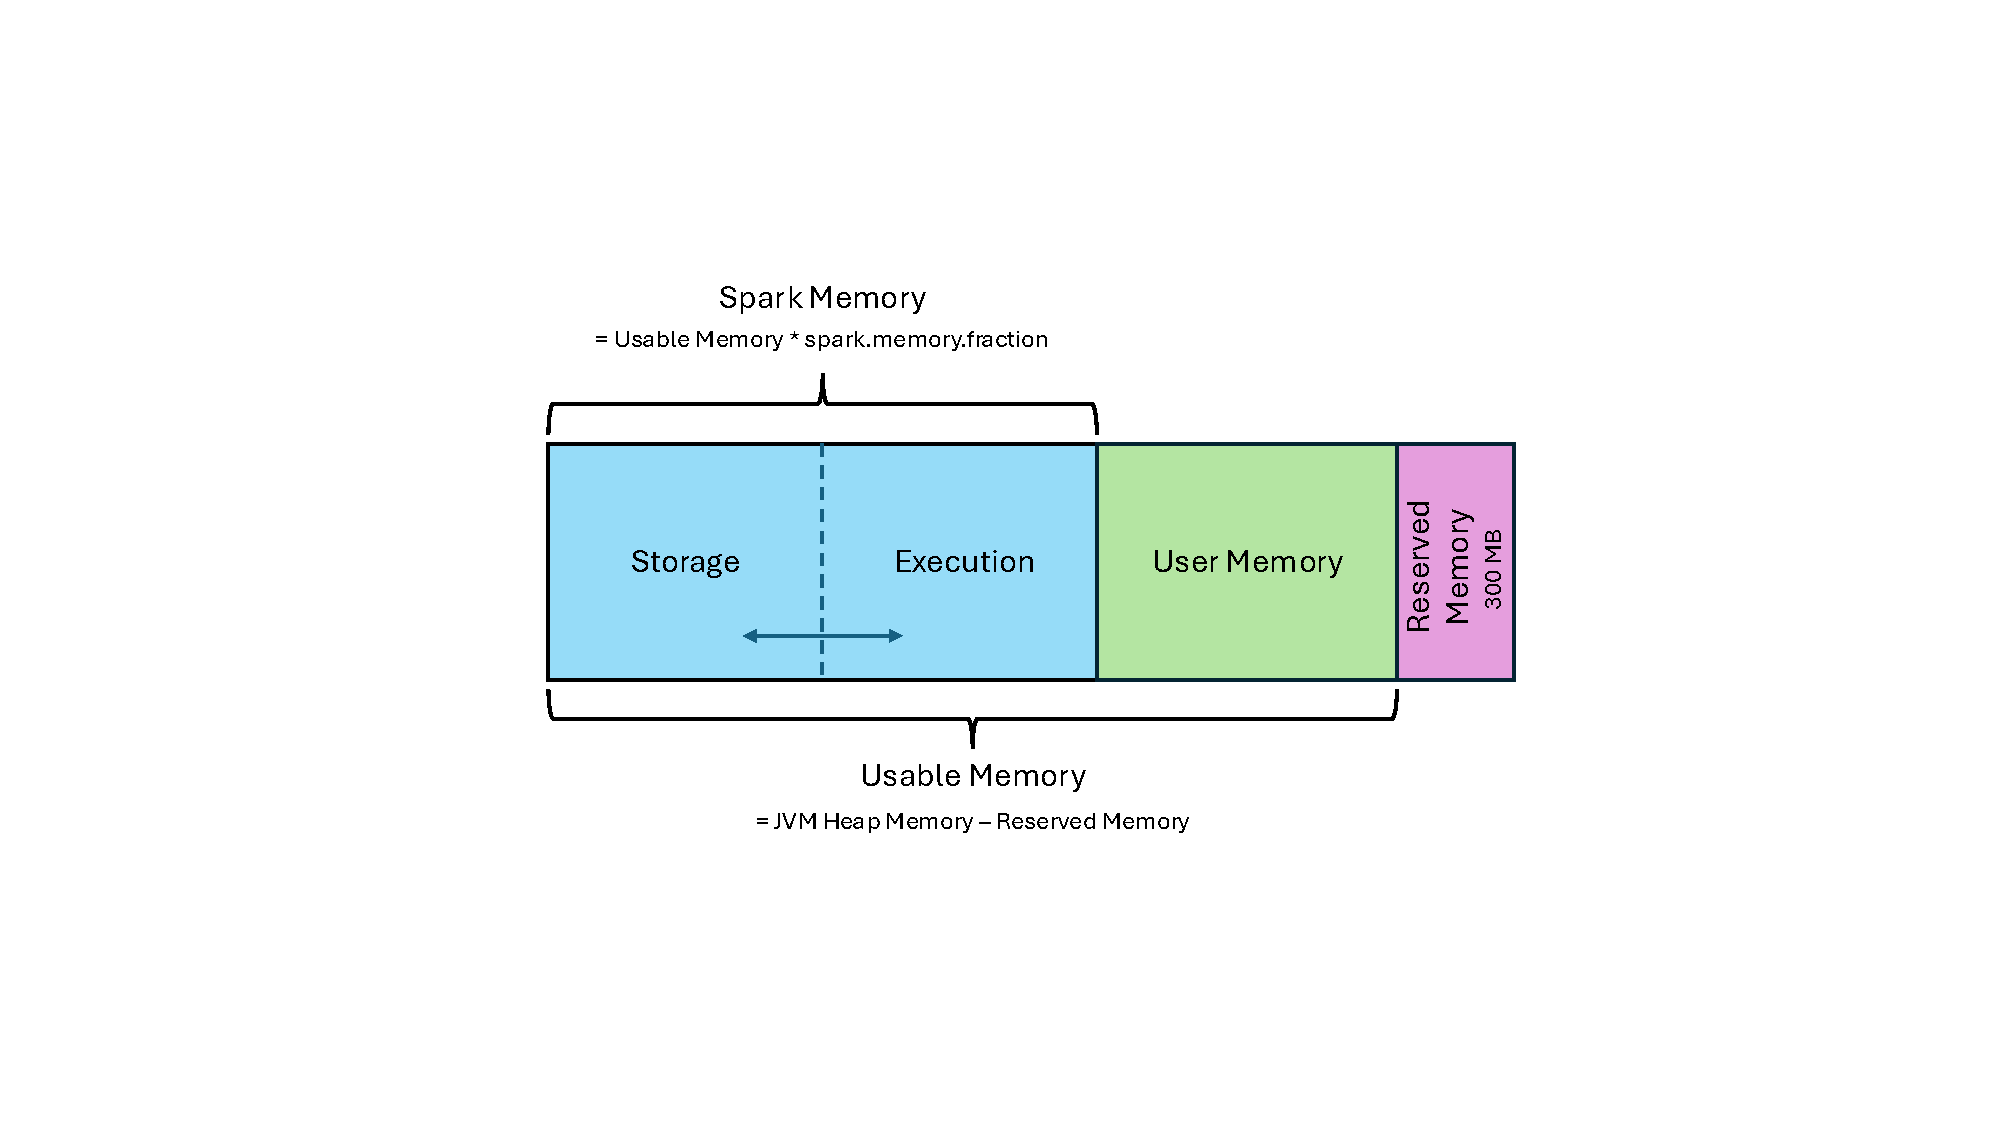
\includegraphics[width=0.7\linewidth]{images/Spark_mem_man.pdf}
    \caption{JVM Heap Memory}
    \label{fig:spark-mem-man}
\end{figure}

\textbf{Reserved Memory.} Of the total memory allocated to an executor, 300 MB are reserved for storing Spark's internal objects. This amount is constant across all executors and guarantees sufficient memory for the system \cite{apache_spark_configuration_2025}.
\textbf{Spark Unified Memory.} This section comprises the usable memory, which is divided into two subregions: \textbf{Spark Memory} and \textbf{User Memory}. The memory allocation depends on spark.memory.fraction. Typically, $0.6$ of the memory is allocated to Spark Memory and $0.4$ to User Memory. Forty percent of the user memory is used to store user data and the results of operations. Spark memory consists of execution and storage memory. Execution memory mainly stores temporary data for computations such as shuffles, joins, and aggregations, while storage memory holds cached data and broadcast variables. Furthermore, the memory allocation between the two can be configured through spark.memory.storage.fraction, where the default value is $0.5$. A special feature of Spark memory is its flexibility. Spark allows executor and storage memory to borrow from each other. This is called the dynamic occupancy mechanism. However, this feature has some limitations. Storage memory can borrow as much execution memory as needed when execution memory is idle. Execution memory, however, can only borrow up to a certain threshold called onHeapStorageSize. Storage memory only uses this part when it's not occupied by execution memory. Storage memory cannot evict execution memory and must wait until it is free. Conversely, execution memory has priority and can evict borrowed memory. In that case, cached data will be evicted until sufficient memory is released. This is because executing a task is more critical than cached data. A task can fail if execution results in an Out-of-Memory (OOM) error. Most operations, however, are executed in on-heap memory, which is subject to garbage collection (GC). Spark can move certain operations to off-heap memory to reduce GC overhead. In this case, memory is stored outside the JVM heap, enabling Spark to manage memory more efficiently. This improves performance for larger workloads, but adds a layer of complexity since Spark must handle memory allocation and deallocation. \cite{chambers_spark_2018}\cite{apache_spark_tuning_2025}. 

% \subsection{Resilient Distributed Dataset}

% % \subsubsection{Definition and Properties of RDDs}
% % \subsubsection{Lineage and Fault Tolerance}
% % \subsubsection{Transformations vs. Actions}
% % \subsubsection{Caching and Persistence}
% % \subsubsection{Implications for Iterative Graph Algorithms}

% A Resilient Distributed Dataset (RDD) is the core abstraction in Spark. An RDD is a partitioned collection of elements that is distributed across the nodes of a cluster. It is processed in parallel \cite{apache_spark_rdd_2025}. RDDs are immutable and resilient to failures due to lineage, which is a feature that records all transformations applied to the data. In the event of a node failure, lost data can be recomputed using these records. RDDs can perform two types of operations: transformations and actions. Each transformation, such as map, filter, or join, creates a new RDD. An action, such as, count, triggers execution. RDDs can be cached or persisted in memory to avoid recomputation with each iteration \cite{chambers_spark_2018}. However, since RDDs are immutable, every transformation creates a new RDD. This can easily result in high memory usage, especially when computing iterative graph algorithms, such as PageRank, where each iteration creates new RDDs for vertex properties. 



\subsection{State of the Art: Approximate PageRank}
% Iteration, sampling, matrix approximation, and Monte Carlo approaches.

% \subsubsection{Iteration-Based Methods}
% \subsubsection{Sampling-Based Methods}
% \subsubsection{Matrix Approximation Methods}
% \subsubsection{Monte Carlo Methods}
% \subsubsection{Trade-offs: Accuracy vs. Efficiency}

The standard PageRank method uses power iteration, which requires storing the entire graph structure in memory. The PageRank values are updated with each iteration until convergence. For large graphs, this process is computationally and memory-intensive, rendering it impractical. Therefore, approximate PageRank algorithms have been proposed for practical, large-scale analysis, which trade off accuracy for efficiency \cite{wu_efficient_2024}. The following methods have been introduced:
\textbf{Iteration methods} \cite{xie_parameterized_2023-1}\cite{anikin_efficient_2022} accelerate the standard power iteration but still operate on the whole graph structure \cite{wu_efficient_2024}. 
\textbf{Sampling-based methods} estimate PageRank values by using smaller, sampled subgraphs \cite{bar-yossef_local_2008}\cite{chen_local_2004}. Despite reducing the size of the input data, these methods cannot estimate the PageRank values for the vertices outside the sampled set \cite{wu_efficient_2024}.
\textbf{Matrix approximation methods} use a low-rank approximated transition matrix to estimate PageRank values \cite{liu_fast_2015}\cite{benczur_feasibility_2005}. 
\textbf{Monte Carlo methods} estimate PageRank values by simulating random walks on the graph. Rather than iteratively updating a full rank vector, these models simulate many random walks on the graph \cite{avrachenkov_monte_2007}. A node's value is estimated by the number of walks that end at the vertex. To achieve high accuracy, these methods require a large number of iterations \cite{wu_efficient_2024}. However, the amount of memory required for the simulation can be controlled by the number of concurrent random walkers rather than by the total number of vertices \cite{avrachenkov_monte_2007}. Given the potential memory advantages of controlling the number of random walkers, Monte Carlo methods offer a promising approach for approximating PageRank on a large scale.
\newpage
\section{Approach}
\subsection{Overview}
\subsection{Motivation for Monte Carlo in Spark}
% Why Monte Carlo is a promising approach for memory-efficiency.
% \subsubsection{Limitations of Iterative PageRank}
% \subsubsection{Idea of Monte Carlo Random Walks}
% \subsubsection{Approximation vs. Convergence Trade-off}
% \subsubsection{Advantages in Spark Environments}

The Monte Carlo method is an alternative approach to the traditional PageRank implementation. Instead of iteratively computing the entire rank vector, it focuses on simulating random walks on the graph. In this approach, a specified number of walkers are released per node, and they then traverse the graph according to the "random surfer" model. Similar to the original algorithm, a random surfer follows an outgoing link with probability $\alpha$ or teleports to a random node in the graph with probability $1-\alpha$. Ultimately, the PageRank values are estimated by the relative frequency with which a node was visited by random walkers. The key difference from the iterative approach is that the walkers take a predefined number of steps instead of updating the rank vector until convergence. Thus, the Monte Carlo approach can control memory usage by limiting the number of walkers and steps, making it a promising candidate for approximating the PageRank of large-scale graphs \cite{avrachenkov_monte_2007}. \par
Additionally, estimating PageRank values is sufficient for many applications. For real-world tasks such as website ranking or user recommendation on social networks, the only things of interest are a node's relative importance and the stability of the ranking. Therefore, total convergence of the PageRank vector is unnecessary. The approximate Monte Carlo approach achieves significant memory and computational savings with only a slight loss in accuracy. This balance between performance and accuracy enables graph analytics on graphs that would otherwise be too large to handle.\par
Furthermore, implementing Monte Carlo PageRank in a Spark environment utilizes a distributed data processing framework that includes Spark's Resilient Distributed \allowbreak Datasets (RDDs). This data structure can represent the entire graph and the walker's state at every step. Spark's properties, such as fault tolerance through lineage and efficient in-memory computation, make it a more attractive platform than the iterative PageRank method for evaluating the Monte Carlo PageRank method. Of particular interest is whether the Monte Carlo approach can operate under limited memory conditions while achieving sufficient accuracy and maintaining low variance throughout the ranking. \par
This thesis explores the integration of such an approximate Monte Carlo method in the Spark environment and evaluates it's performance and accuracy on limited memory usage in comparison to the standard GraphX PageRank method.
 

\subsection{Algorithm Design}
% Describe how RDDs are used for graph and walker states.

% \subsubsection{Initialization of Walkers}
% \subsubsection{Step-by-Step Simulation Process}
% \subsubsection{Random Number Generation and Reproducibility}
% \subsubsection{Handling Dangling Nodes}
% \subsubsection{Computation of Approximate PageRank Scores}

The approximate Monte Carlo algorithm estimates the stationary distribution by leveraging a step by step simulation that follows the random surfer model.
The pseudo code bellow presents the walker simulation and the decision logic used in each step.

\vspace{1.5em}
\begin{algorithm}[H]
\caption{Monte Carlo PageRank Approximation}
\KwIn{Graph $G=(V,E)$, walkers per node $w$, number of steps $k$, damping factor $\alpha$}
\KwOut{Approximate PageRank scores $\hat{\pi}(v)$ for all $v \in V$}

\ForEach{node $v \in V$}{
Initialize $w$ walkers at $v$
}
\For{step = 1 to $k$}{
\ForEach{walker $i$ at node $u$}{
Generate random number $r \in [0,1]$;
\eIf{$r < \alpha$ \textbf{and} $u$ has outgoing edges}{
Move walker to a random neighbor of $u$;
}{
Teleport walker to a random node $v \in V$;
}
}
}
\ForEach{node $v \in V$}{
$\hat{\pi}(v) \gets \frac{\text{Number of walkers at } v}{|V| \cdot w}$
}
\end{algorithm}
\vspace{1.5em}

The algorithm initializes $w$ walkers per node, which is resulting in a total number of $w\cdot |V|$ walkers. Each walker is randomly distributed throughout the graph. Then, each walker simultaneously performs a number of $k$ independent steps.
At each step, the walker $w$ generates a random number between $0$ and $1$. To ensure deterministic behavior, each walker uses a seeded random number generator that guarantees reproducibility:

\vspace{0.5em}
\newpage
\begin{lstlisting}[caption={Materializing and Unpersisting Walker RDD},
                   label={lst:walker},
                   captionpos=b] 
val seed = System.nanoTime + Thread.currentThread().getId + step + currentNode.toInt
\end{lstlisting}


\vspace{0.5em}

In case a node does not have any outedges, it's treated as a dangling node and the walker will directly teleport to a random node.
After $k$ steps the simulation terminates and the PageRank values are approximated based on the walker visits of a node.

\subsection{Implementation in Spark}
% \subsubsection{Graph Representation with RDDs}
% \subsubsection{Adjacency List Construction}
% \subsubsection{Broadcasting for Teleportation}
% \subsubsection{Walker State Representation and Distribution}
% \subsubsection{RDD Caching, Materialization, and Unpersisting}
% \subsubsection{Repartitioning for Load Balancing}

The Monte Carlo Implementation is structured around two main components: The graph representation and the walker states. Both of them are stored in Sparks RDDs, which make them suitable for processing in a distributed system.

At the beginning of the program a given edge list file is read to get the structure of the graph. It is stored as an RDD of directed edges. Then by grouping the outgoing neighbors of each node an adjacency list is constructed, which is one of the main RDD-based components, that is represnting the entire graph structure:

\vspace{0.5em}
\begin{lstlisting}[language=Scala, caption={Adjacency list creation}, label={lst:adjlist}]
val adjList: RDD[(Long, Iterable[Long])] = edgesRDD.groupByKey().cache()
\end{lstlisting}
\vspace{0.5em}

Additionally, an array of all vertices is required to support teleportation. This list will be distributed as a broadcasting variable to all nodes.

\vspace{0.5em}
\begin{lstlisting}[language=Scala, caption={Broadcasting Variable}, label={lst:broadcast}]
val broadcastNodes = sc.broadcast(allNodesArray)
\end{lstlisting}
\vspace{0.5em}

This mitigates costly network shuffles during every teleportation. Because the set of nodes is required in every simulation step it is cached in memory for efficient access.
A fixed number of walkers are initialized and represented in a seperate RDD. The RDD is distributed across multiple partitions to ensure efficient parallel processing and scaling when analyzing large graphs. Each entry in the RDD is a random vertex ID, representing the current vertex of a walker. In each simulation step the walker RDD is joined with the adjacency list to get all possible outgoing edges. After each walker updates its position, a new walker RDD is initialized with the updated positions. Before the previous walker RDD is explicitly unpersisted after the step is completed, the new walker RDD has to be materialized.
\newpage
\begin{lstlisting}[language=Scala, caption={Materializing and Unpersisting Walker RDD}, label={lst:materialize}]
nextWalkersRDD.cache() 
nextWalkersRDD.count() // trigger an action to materialze RDD
walkersRDD.unpersist(blocking = false)
\end{lstlisting}
\vspace{0.5em}
This is because Spark uses lazy evaluation. It ensures that only the current walker RDD and the adjacency list occupy memory. \par
Before caching the walkers RDD in memory, repartitioning is applied to the RDD after each step. This is crucial for balanced distribution across partitions as it ensures that the number of partitions remains the same throughout the experiment. 
When processing large graphs that include nodes with high ingoing edges it prevents skews and stragglers allowing Spark to efficiently use all available cores. Managing the partitions correctly can have a significant impact on performance. 


\subsection{Experimental Framework and Automation}

% \subsubsection{Datasets: Real-World and Synthetic Graphs}
% \subsubsection{Synthetic Graph Generation}
% \subsubsection{Parameter Variation in Experiments}
% \subsubsection{Spark Cluster Setup}
% \subsubsection{Automation via Shell Scripts}
% \subsubsection{Data Collection and Visualization}

Finally, to evaluate the performance of the approximate Monte Carlo method an experimental framework was established, that aims for reproducibility. It benchmarks the Monte Carlo method and compares it to the standard PageRank method. The evaluation is focusing mainly on memory efficiency while trading off performance and accuracy. \par
The datasets used for evaluation include both real-world and synthetic graphs. Real-world graphs such as wiki-Talk provide an irregular graph structure and millions of edges, presenting a practical use case. On the other hand, synthetic graphs of any size and with different characteristics can be generated. In the experiments, Erdős–Rényi graphs of different sizes, ranging from $100.000$ to $20$ million nodes, have been generated. To establish comparable conditions between the different graph sizes, the density is kept consistent by controlling the number of outgoing edges per node. However, the in-degree of each node is random and ranges between $0$ and $n-1$, where $n$ is the total number of nodes. A simple python script is used to generate and store the graph structure in an edge list file.

\vspace{1.5em}
\begin{algorithm}[H]
\caption{Synthetic Graph Generator}
\KwIn{Range of node counts $[N_{\min}, N_{\max}]$, step size $\Delta N$, edges per node $E$}
\KwOut{Synthetic graph files with $E$ outgoing edges per node}

Set random seed for reproducibility\;
\For{$n \gets N_{\min}$ \KwTo $N_{\max}$ \KwStep $\Delta N$}{
  Create output file for graph with $n$ nodes\;
  \ForEach{node $u \in \{1, \dots, n\}$}{
    \For{$i \gets 1$ \KwTo $E$}{
      Select random destination $v \in \{1, \dots, n\}$\;
      \If{$v \neq u$}{
        Write edge $(u, v)$ to file\;
      }
    }
  }
  
}
\end{algorithm} 
\vspace{1.5em}

The output can be directly used for Spark processing.\par
During the experiments, the main parameters of the Monte Carlo method have been varied. The parameters include the number of walkers and the number of steps per walker. The goal was to systematically compare performance, memory and runtime across varying parameters. In the GraphX implementation the only parameters that were configured are the tolerance and the damping factor. The tolerance is usually set to $0.001$. In the experiments it was kept on such a low value to get very precise PageRank values and to compare the approximate Monte Carlo approach to the standard PageRank method. The reset probability was set to $0.15$ for both methods. Additionally, different Spark configurations were analyzed such as the number of executors and most importantly the memory allocated per executor. \par



To automate the experiments, shell scripts are used. Each script relies on spark-submit, which is the standard command line tool used to launch applications on a Spark cluster. In the spark-submit command configurations such as the number of executors and the memory per executor can be set. Furthermore, the edge list file is passed to the script as well as the Monte Carlo specific configuration such as the number of walkers and steps per walker. This setup ensures that experiments are running in a sequence without needing manual input and with consistency throughout multiple data sets. Finally, the spark-submit command allows to either run the applications locally or to launch them to a cluster environment to simulate a real distributed system. \par

To ensure comparable conditions across all experiments, all experiments are executed on a Spark cluster set up on the university's server. For simplicity, the Spark cluster is deployed in standalone mode, which is a built-in cluster manager. Only the master and workers need to be started on the university server. The cluster consists of one master node and four worker nodes. Each worker node has one executor with two cores, for a total of eight cores. \par


In every experiment, metrics for both methods are collected, including configurations such as the number of walkers and steps for the Monte Carlo method. Another file collects the total runtime, allocated memory, and graph size to evaluate performance with limited memory and with different graph sizes. For accuracy evaluation, the top 20 ranks for both methods are saved in a separate file. \par
All the collected data is saved in CSV files to efficiently analyze it in the next step. With the help of Python scripts and the use of libraries such as Matplotlib and Pandas, the data is structured and visualized in various plots of runtime, allocated memory, accuracy and cost. This provides a clear overview of the data and enables a thorough analysis of the data. \par
This setup ensures the reproducibility and scalability of evaluating the Monte Carlo method. This is achieved through the use of various datasets, such as real-world and synthetic data, as well as a systematic variation in parameters. Additionally, scripts automate experiments and efficiently collect key metrics. This framework enables the analysis of the empirical results presented in the following sections. \par
\begin{figure}[H]
    \centering
    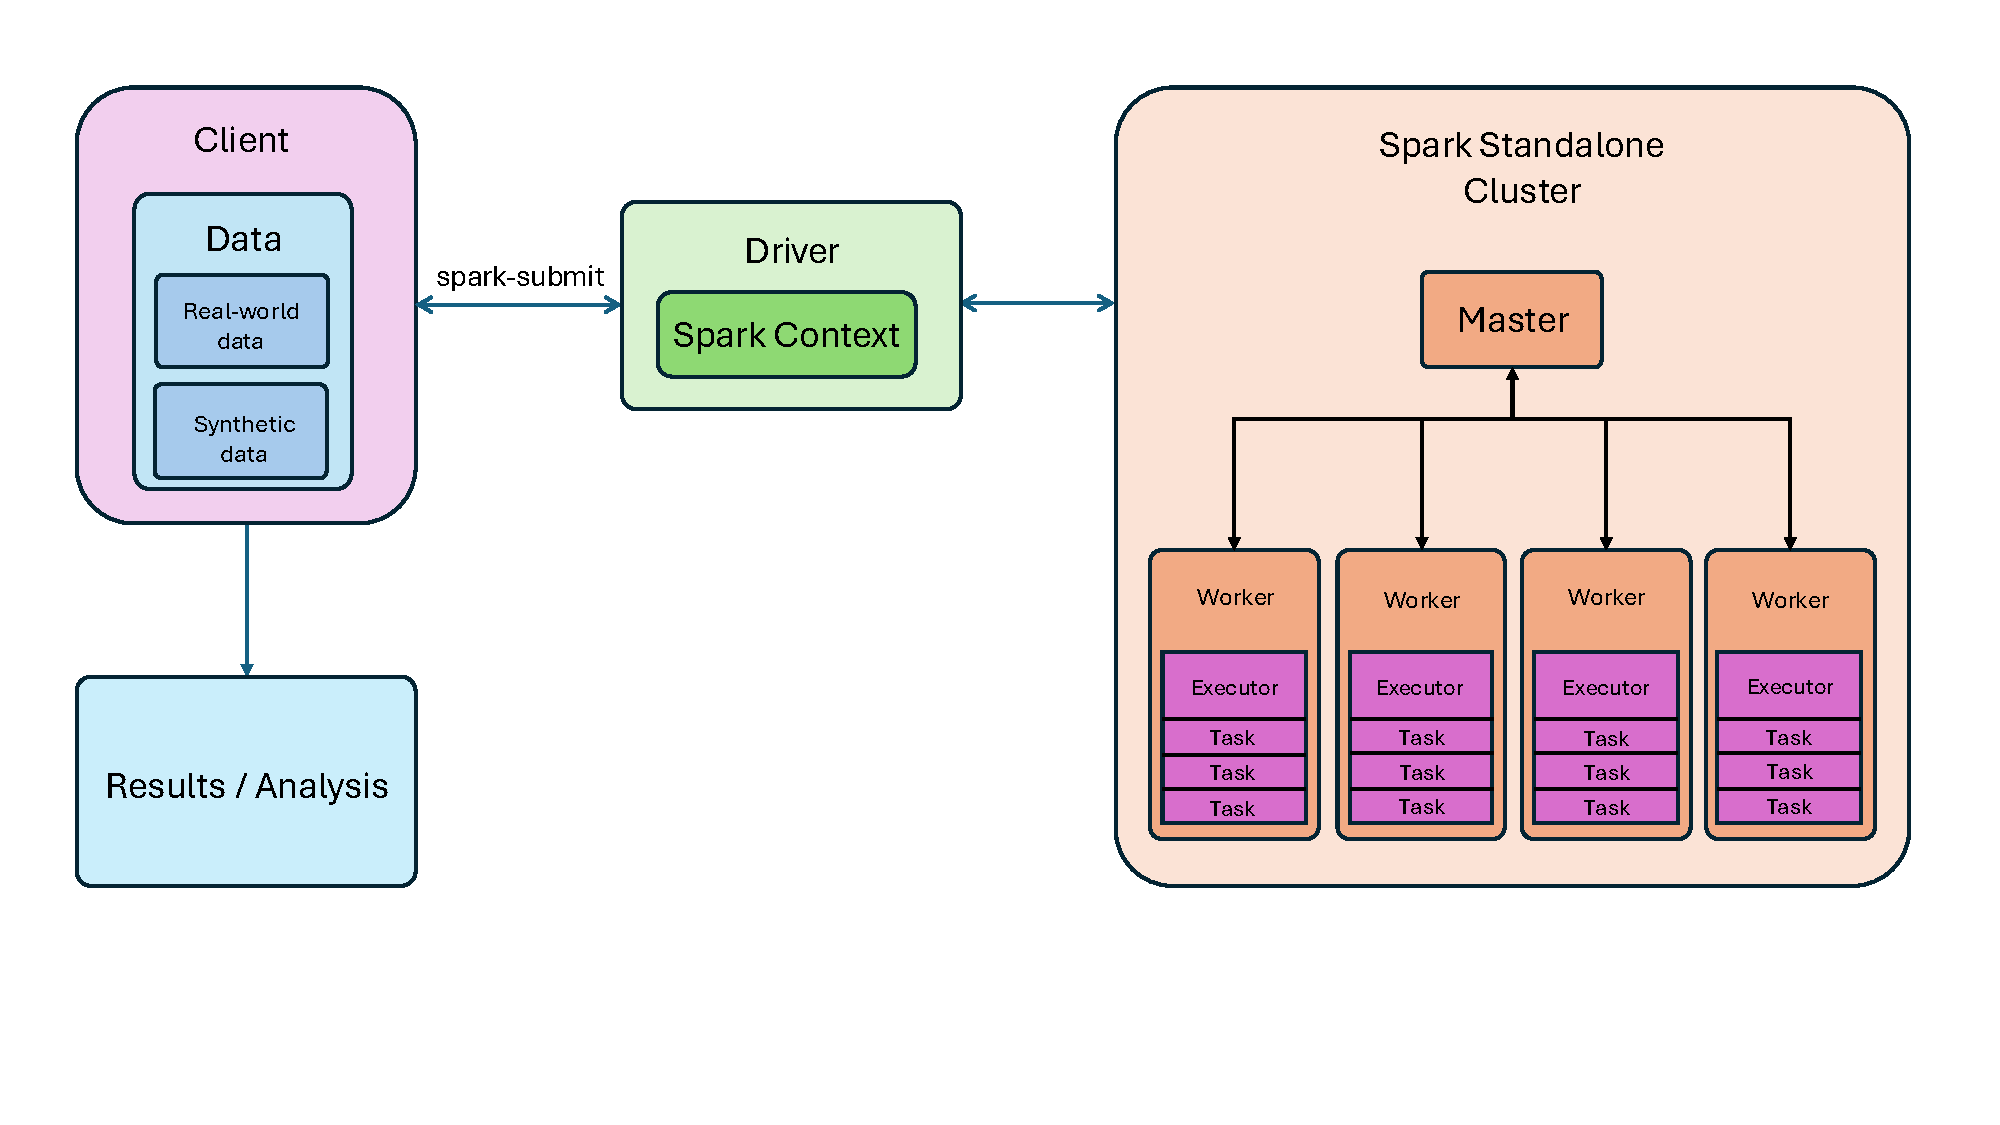
\includegraphics[width=\linewidth]{images/Workflow_image.pdf}
    \caption{Experimental Workflow}
    \label{fig:workflow}
\end{figure}
Finally, the given approach combines an approximate Monte Carlo implementation with a distributed Spark environment and a systematic experimental framework. The main goal of this setup is to determine whether the described method can operate with much less memory than the standard PageRank implementation. While a trade-off in accuracy and performance is expected and tolerated, the method aims to provide sufficient accuracy and performance. The evaluation will reveal whether the Monte Carlo approach is a viable alternative to the standard PageRank method in environments with restricted memory and large-scale graphs, addressing the central research question of this thesis.


\subsection{Error Handling}
% \subsubsection{Out-of-Memory Handling}
% \subsubsection{Crash Scenarios Encountered During Experiments}
% \subsubsection{Timeout: How and when to cancel an Experiment}

When processing large-scale graphs, memory exhaustion and application crashes are inevitable. Therefore, error-handling strategies are necessary to ensure that experiments remain reproducible and manageable. For simplicity, this thesis only differentiates between out-of-memory (OOM) failures and timeouts. \par
The Java Out-of-Memory exception is a common scenario that is expected in this experimental setup because the goal is to deliberately strain memory. This exception is usually thrown when there is not enough memory in the Java heap to allocate to an object. This means the garbage collector is unable to free up enough space for the object. In these experiments, the exception was detected in the log files. In that case, the configurations are automatically marked as failed and excluded from further experiments. \par
Since very large graphs are being processed, some experiments can take a disproportionately long time to finish. This is why a timeout mechanism is implemented to prevent experiments from blocking the pipeline. If an experiment does not finish within the predefined time, the current experiment is terminated, and the next experiment with different configurations begins. This ensures that all experiments finish within an acceptable time frame.  \par
These error handling strategies establish a more systematic and stable process. Experiments can run without manual intervention, and the resulting datasets are more consistent.


\newpage
\section{Evaluation}
\subsection{Datasets}
 Both real-world and synthetic datasets were used to evaluate and compare the approximate Monte Carlo method to the standard PageRank method. The real-world datasets were obtained from the Stanford Network Analysis Project (SNAP), a well-known repository of large graph datasets \cite{standford_university_snap_2025}. It includes social networks, web graphs, and communication networks, among others. These datasets such as wiki-Talk are publicly available and can be downloaded from the SNAP website. These graphs have realistic structures with millions of nodes and edges. \par
Furthermore, synthetic graphs of any size and with different characteristics can be generated. In the experiments, Erdős–Rényi graphs of different sizes, ranging from $100.000$ to $20$ million nodes, have been generated. To establish comparable conditions between the different graph sizes, the density is kept consistent by controlling the number of outgoing edges per node. However, the in-degree of each node is random and ranges between $0$ and $n-1$, where $n$ is the total number of nodes. A simple python script was used to generate and store the graph structure in an edge list file.

\vspace{1.0em}
\begin{algorithm}[H]
\caption{Synthetic Graph Generator}
\KwIn{Range of node counts $[N_{\min}, N_{\max}]$, step size $\Delta N$, edges per node $E$}
\KwOut{Synthetic graph files with $E$ outgoing edges per node}

Set random seed for reproducibility\;
\For{$n \gets N_{\min}$ \KwTo $N_{\max}$ \KwStep $\Delta N$}{
  Create output file for graph with $n$ nodes\;
  \ForEach{node $u \in \{1, \dots, n\}$}{
    \For{$i \gets 1$ \KwTo $E$}{
      Select random destination $v \in \{1, \dots, n\}$\;
      \If{$v \neq u$}{
        Write edge $(u, v)$ to file\;
      }
    }
  }
  
}
\end{algorithm} 
\vspace{1.0em}

The selected datasets from SNAP vary in size, structure and density. The following table presents the chosen graphs and their characteristics: 

% include table
\begin{table}[ht]
\centering
\setlength{\tabcolsep}{6pt}
\renewcommand{\arraystretch}{1.2}
\begin{tabularx}{\linewidth}{l r r l X}
\toprule
\textbf{Dataset} & \textbf{Nodes} & \textbf{Edges} & \textbf{Type} & \textbf{Expected Behavior} \\
\midrule
wiki-Talk    & 2.4M & 5M    & Communication & Medium convergence \\
web-Google   & 875K & 5.1M  & Web Graph & Fast convergence, extreme authority \\
soc-Pokec    & 1.6M & 30.6M & Social Network & Slow convergence, distributed authority \\
web-BerkStan & 685K & 7.6M  & Web Graph & Fast convergence, dense connections \\
\bottomrule
\end{tabularx}
\caption{Benchmark datasets and expected behavior.}
\label{tab:datasets}
\end{table}



 %The real-world datasets selected from SNAP vary in size, density, and structure. Among them are:

%Wiki-Talk: A communication network from Wikipedia where a directed edge from user u to user v indicates that u has edited v’s talk page. This dataset contains millions of edges and is highly irregular, with some users having extremely high degree. It is one of the largest and most challenging graphs used in the experiments.

% Wiki-Vote: A voting network of Wikipedia users where edges represent votes cast in administrator elections. The dataset is smaller but directed, providing a good comparison for medium-sized graphs.

% Slashdot: A social network where edges represent “friend” or “foe” relationships between users. This dataset is useful because it represents a signed social graph with complex structure.

% Amazon Co-Purchasing Network: A product co-purchasing network where nodes are products and edges indicate that two products are often bought together. This dataset models a recommendation-style graph and offers a different type of degree distribution.


%\subsubsection{Data Sources of real-world Graphs}
% Description of synthetic and real-world datasets used


\subsection{Implementation in Spark}
% \subsubsection{Graph Representation with RDDs}
% \subsubsection{Adjacency List Construction}
% \subsubsection{Broadcasting for Teleportation}
% \subsubsection{Walker State Representation and Distribution}
% \subsubsection{RDD Caching, Materialization, and Unpersisting}
% \subsubsection{Repartitioning for Load Balancing}

The Monte Carlo Implementation is structured around two main components: The graph representation and the walker states. Both of them are stored in Sparks RDDs, which make them suitable for processing in a distributed system.\par

At the beginning of the program an edge list file is read to get the structure of the graph. It is stored as an RDD of directed edges. Then by grouping the outgoing neighbors of each node an adjacency list is constructed, which is one of the main RDD-based components, that is represnting the entire graph structure:

\vspace{0.5em}
\begin{lstlisting}[language=Scala, caption={Adjacency list creation}, label={lst:adjlist}]
val adjList: RDD[(Long, Iterable[Long])] = edgesRDD.groupByKey().cache()
\end{lstlisting}
\vspace{0.5em}

Additionally, an array of all vertices is required to support teleportation. This list will be distributed as a broadcasting variable to all nodes.

\vspace{0.5em}
\begin{lstlisting}[language=Scala, caption={Broadcasting Variable}, label={lst:broadcast}]
val broadcastNodes = sc.broadcast(allNodesArray)
\end{lstlisting}
\vspace{0.5em}

This mitigates costly network shuffles during every teleportation. Because the set of nodes is required in every simulation step it is cached in memory for efficient access.
A fixed number of walkers are initialized and represented in a seperate RDD. The RDD is distributed across multiple partitions to ensure efficient parallel processing and scaling when analyzing large graphs. Each entry in the RDD is a random vertex ID, representing the current vertex of a walker. In each simulation step the walker RDD is joined with the adjacency list to get all possible outgoing edges. After each walker updates its position, a new walker RDD is initialized with the updated positions. Before the previous walker RDD is explicitly unpersisted after the step is completed, the new walker RDD has to be materialized.
%\newpage
\begin{lstlisting}[language=Scala, caption={Materializing and Unpersisting Walker RDD}, label={lst:materialize}]
nextWalkersRDD.cache() 
nextWalkersRDD.count() // trigger an action to materialze RDD
walkersRDD.unpersist(blocking = false)
\end{lstlisting}
\vspace{0.5em}
This is because Spark uses lazy evaluation. It ensures that only the current walker RDD and the adjacency list occupy memory. \par
Before caching the walkers RDD in memory, repartitioning is applied to the RDD after each step. This is crucial for balanced distribution across partitions as it ensures that the number of partitions remains the same throughout the experiment. 
When processing large graphs that include nodes with high ingoing edges it prevents skews and stragglers allowing Spark to efficiently use all available cores. Managing the partitions correctly can have a significant impact on performance. 


\subsection{Experimental Framework and Automation}

% \subsubsection{Datasets: Real-World and Synthetic Graphs}
% \subsubsection{Synthetic Graph Generation}
% \subsubsection{Parameter Variation in Experiments}
% \subsubsection{Spark Cluster Setup}
% \subsubsection{Automation via Shell Scripts}
% \subsubsection{Data Collection and Visualization}

To evaluate the performance of the approximate Monte Carlo method an experimental framework was established, that aims for reproducibility. It benchmarks the Monte Carlo method and compares it to the standard PageRank method. The evaluation is focusing mainly on memory efficiency while trading off performance and accuracy. \par
% The datasets used for evaluation include both real-world and synthetic graphs. Real-world graphs such as wiki-Talk provide an irregular graph structure and millions of edges, presenting a practical use case. On the other hand, synthetic graphs of any size and with different characteristics can be generated. In the experiments, Erdős–Rényi graphs of different sizes, ranging from $100.000$ to $20$ million nodes, have been generated. To establish comparable conditions between the different graph sizes, the density is kept consistent by controlling the number of outgoing edges per node. However, the in-degree of each node is random and ranges between $0$ and $n-1$, where $n$ is the total number of nodes. A simple python script is used to generate and store the graph structure in an edge list file.

% \vspace{1.5em}
% \begin{algorithm}[H]
% \caption{Synthetic Graph Generator}
% \KwIn{Range of node counts $[N_{\min}, N_{\max}]$, step size $\Delta N$, edges per node $E$}
% \KwOut{Synthetic graph files with $E$ outgoing edges per node}

% Set random seed for reproducibility\;
% \For{$n \gets N_{\min}$ \KwTo $N_{\max}$ \KwStep $\Delta N$}{
%   Create output file for graph with $n$ nodes\;
%   \ForEach{node $u \in \{1, \dots, n\}$}{
%     \For{$i \gets 1$ \KwTo $E$}{
%       Select random destination $v \in \{1, \dots, n\}$\;
%       \If{$v \neq u$}{
%         Write edge $(u, v)$ to file\;
%       }
%     }
%   }
  
% }
% \end{algorithm} 
% \vspace{1.5em}

\par
During the experiments, the main parameters of the Monte Carlo method have been varied. The parameters include the number of walkers and the number of steps per walker. The goal was to systematically compare performance, memory and runtime across varying parameters. In the GraphX implementation the only parameters that were configured are the tolerance and the damping factor. The tolerance is usually set to $0.001$. In the experiments it was kept on such a low value to get very precise PageRank values and to compare the approximate Monte Carlo approach to the standard PageRank method. The reset probability was set to $0.15$ for both methods. Additionally, different Spark configurations were analyzed such as the number of executors and most importantly the memory allocated per executor. \par



To automate the experiments, shell scripts are used. Each script relies on spark-submit, which is the standard command line tool used to launch applications on a Spark cluster. In the spark-submit command configurations such as the number of executors and the memory per executor can be set. Furthermore, the edge list file is passed to the script as well as the Monte Carlo specific configuration such as the number of walkers and steps per walker. This setup ensures that experiments are running in a sequence without needing manual input and with consistency throughout multiple data sets. Finally, the spark-submit command allows to either run the applications locally or to launch them to a cluster environment to simulate a real distributed system. \par

\begin{figure}[H]
    \centering
    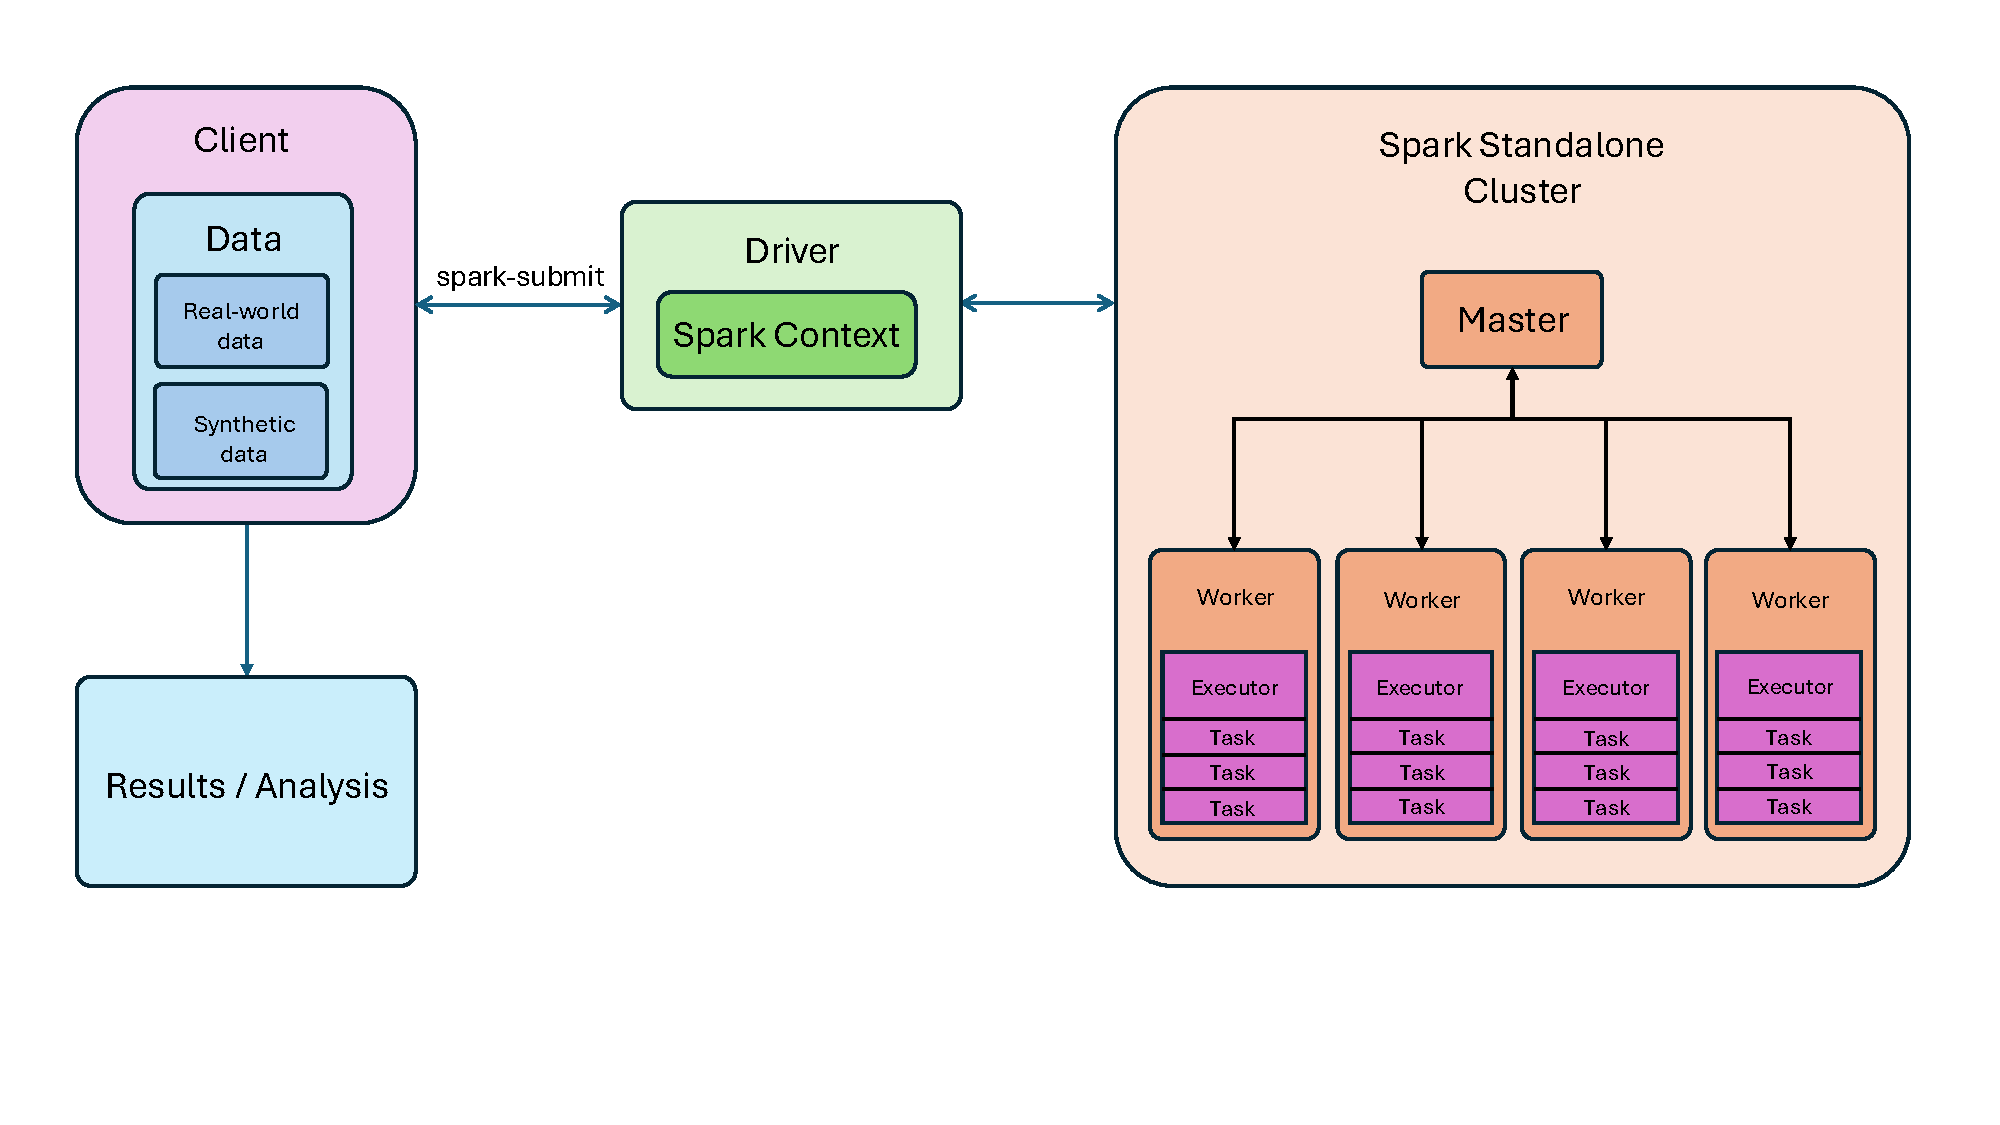
\includegraphics[width=\linewidth]{images/Workflow_image.pdf}
    \caption{Experimental Workflow}
    \label{fig:workflow}
\end{figure}
To ensure comparable conditions across all experiments, all experiments were executed on a Spark cluster set up on the university's server. For simplicity, the Spark cluster was deployed in standalone mode, which is a built-in cluster manager. Only the master and workers need to be started on the university server. The cluster consists of one master node and four worker nodes. Each worker node has one executor with two cores, for a total of eight cores. \par


In every experiment, metrics for both methods were collected, including configurations such as the number of walkers and steps for the Monte Carlo method. Another file collected the total runtime, allocated memory, and graph size to evaluate performance with limited memory and with different graph sizes. For accuracy evaluation, the top 20 ranks for both methods were saved in a separate file. \par
All the collected data was saved in CSV files to efficiently analyze it in the next step. With the help of Python scripts and the use of libraries such as Matplotlib and Pandas, the data is structured and visualized in various plots of runtime, allocated memory, accuracy and cost. This provides a clear overview of the data and enables a thorough analysis of the data. \par
This setup ensures the reproducibility and scalability of evaluating the Monte Carlo method. This was achieved through the use of various datasets, such as real-world and synthetic data, as well as a systematic variation in parameters. Additionally, scripts automated experiments and efficiently collected key metrics. This framework enabled the analysis of the empirical results presented in the following sections. \par
% \begin{figure}[H]
%     \centering
%     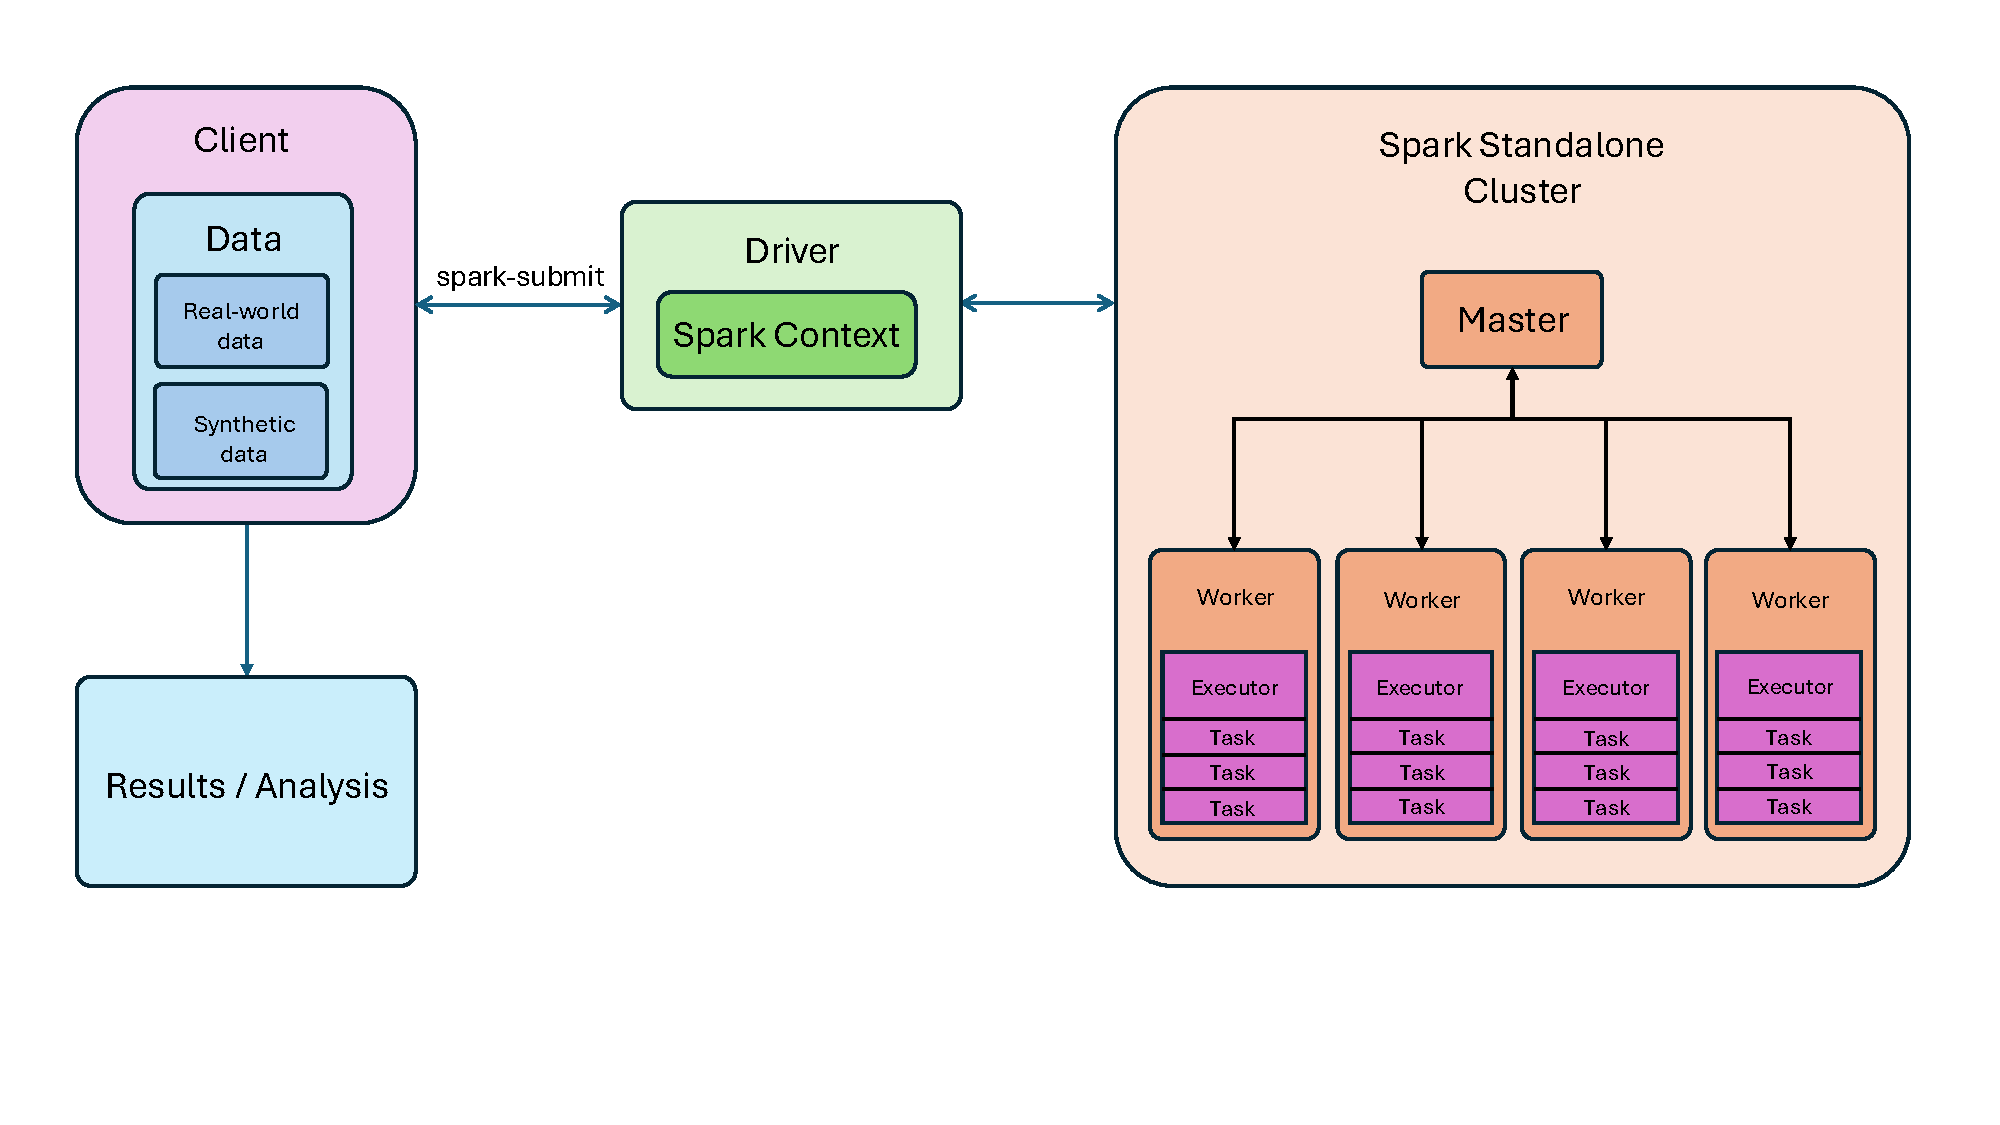
\includegraphics[width=\linewidth]{images/Workflow_image.pdf}
%     \caption{Experimental Workflow}
%     \label{fig:workflow}
% \end{figure}
Finally, the given approach combines an approximate Monte Carlo implementation with a distributed Spark environment and a systematic experimental framework. The main goal of this setup was to determine whether the described method can operate with much less memory than the standard PageRank implementation. While a trade-off in accuracy and performance was expected and tolerated, the method aims to provide sufficient accuracy and performance. The evaluation will reveal whether the Monte Carlo approach is a viable alternative to the standard PageRank method in environments with restricted memory and large-scale graphs, addressing the central research question of this thesis.


\subsection{Error Handling}
% \subsubsection{Out-of-Memory Handling}
% \subsubsection{Crash Scenarios Encountered During Experiments}
% \subsubsection{Timeout: How and when to cancel an Experiment}

When processing large-scale graphs, memory exhaustion and application crashes are inevitable. Therefore, error-handling strategies were necessary to ensure that experiments remain reproducible and manageable. For simplicity, this thesis only differentiates between out-of-memory (OOM) failures and timeouts. \par
The Java Out-of-Memory exception is a common scenario that was expected in this experimental setup because the goal was to deliberately strain memory. This exception is usually thrown when there is not enough memory in the Java heap to allocate to an object. This means the garbage collector is unable to free up enough space for the object. In these experiments, the exception was detected in the log files. In that case, the configurations were automatically marked as failed and excluded from further experiments. \par
Since very large graphs were being processed, some experiments can take a disproportionately long time to finish. This is why a timeout mechanism was implemented to prevent experiments from blocking the pipeline. If an experiment did not finish within the predefined time, the current experiment was terminated, and the next experiment with different configurations started. This ensures that all experiments finished within an acceptable time frame.  \par
These error handling strategies established a more systematic and stable process. Experiments could run without manual intervention, and the resulting datasets are more consistent.

% \subsection{Datasets}
 


% \subsubsection{Data Sources of real-world Graphs}
% % Description of synthetic and real-world datasets used.

\subsection{Allocated Memory}
The main goal of this thesis was to investigate wether the Monte Carlo PageRank approach is able to operate on restrained memory and compare it to the standard PageRank approach. Therefore, allocated memory was analyzed as the key evaluation metric. 
\vspace{0.5em}
\begin{lstlisting}[language=bash, caption={Spark-submit command}]
spark-submit \
  --class "$SPARK_APP_CLASS" \
  --master spark://casa-ubu.eecsit.tu-berlin.de:7077 \
  --name "Demo-$base-$EXECUTOR_MEM" \
  --deploy-mode client \
  --driver-memory 3g \
  --executor-cores 2 \
  --conf spark.cores.max=8 \
  --executor-memory "$EXECUTOR_MEM" \
\end{lstlisting}
\vspace{0.5em}
In Spark, the executor memory is allocated through spark-submit, which is shown above. The parameter executor-memory specifies the available JVM heap size per executor. For all experiments the allocated memory per executor was varied and set between 450 MiB and 8 GiB. Other parameters such as the number of executors and total numbers of cores were kept the same to ensure comparability throughout all experiments.\par
The memory configurations were logged for both the Monte Carlo method and the standard method. In case the allocated memory was not sufficient for the application and an OOM exception was thrown, the error was handled as mention above. The failed runs show the boundaries of each method under limited memory. The focus of the analysis is put on the minimum memory required and how this changes with increasing the graph size. The results are comapred between the two methods.



\subsection{Runtime}
Runtime is another metric that was analyzed in this thesis. It shows how both methods perform under limited memory conditions. Although a trade-off in runtime was considered as acceptable, the methods should aim to finish within an acceptable time under the given circumstances. It also shows the practicality of both methods.\par
Therefore, a timeout of 30 minutes was implemented and the experiments were handled according to the error handling section.\par 
The total runtime of each experiment was measured from when the Spark application was submitted until the Spark Session was stopped. The shell scripts that automated the experiments also logged the runtime and the configurations, which ensures an identical setup across all experiments.\par
The analyses focuses mainly on the effect of different graph sizes on the runtime. 


\subsection{Accuracy}
The accuracy was evaluated by comparing the ranks of the Monte Carlo method and the standard PageRank method. The standard PageRank method is considered to be the ground truth as it was configured with a tolerance of $0.001$. During the experiments the goal was to determine how close ranks are to the ground truth. Accuracy is mainly controlled by the number of walkers, the steps per walker and the graph structure. \par

Since in many real-world applications only the top ranks are needed, the goal was to only analyze the top $20$ ranks. The ranks were also collected through the shell scripts. The accuracy was then determined by the Jaccard index, which is a statistic used to measure the similarity and distance of sample sets. Jaccard index in combination with the top $20$ ranks is very simple and focuses on overlap of important nodes instead of overemphasizing tail nodes.

\vspace{1.0em}
\begin{algorithm}[H]
\caption{Jaccard Similarity}
\KwIn{Two rank lists $L_{MC}$, $L_{GX}$}
\KwOut{Similarity $s$, Distance $d$}

$S_{MC} \gets$ set($L_{MC}$) \;
$S_{GX} \gets$ set($L_{GX}$) \;

$I \gets |S_{MC} \cap S_{GX}|$ \;  
$U \gets |S_{MC}| + |S_{GX}| - I$ \; 

$s \gets I / U$ \;
$d \gets 1 - s$ \;

\Return $(s, d)$ \;
\end{algorithm}
\vspace{1.0em}

The resulting value is a percentage that represents the similarity to the ground truth. \par

The accuracy was analyzed on different graph sizes and structures. Additionally the number of walkers and the number of steps was varied across experiments. With an increasing number of walkers and steps a higher accuracy was expected. Furthermore larger and more complex graphs would require more walkers to achieve good accuracy. Also, a variance in the ranks of the Monte Carlo approach was expected since it follows the random surfer model and identical ranks are unlikely. Therefore, the average similarity of the top $20$ ranks across five different runs with the same configurations was taken to get a more representative result.


\subsection{Costs (GiB-hours)}
% Memory usage, runtime, accuracy (e.g., compared to GraphX).
A cost metric was introduced to reflect both runtime and minimal allocated memory. GiB-hours combines these two metrics to show how much cluster memory was allocated and for how long. It is the area under the memory time curve. For each experiment, it was computed by multiplying the allocated executor memory (GiB) by the runtime (hours). \par
Since the setup was constant across all experiments, the cost metric was primarily influenced by executor memory and runtime. The driver memory was also kept constant to maintain focus on executor memory during the experiments and to make to GiB-hours directly comparable across Monte Carlo and GraphX experiments. Additionally, no off-heap or reserved memory was added. Thus, the cost metric depends solely on the configured on-heap executor memory. However, GiB-hours doesn't capture all costs such as the network costs.\par
If only the runtime had been taken into account, the experiments with high memory demand would have appeared to be more favorable, even though they consumed much more memory. This is why the cost metric is crucial for providing a balanced overview. It captures both runtime and memory usage during the experiment. \par
The analysis predicted that the Monte Carlo approach would require fewer GiB-hours, while the standard PageRank method was expected to be significantly more costly.


\subsection{Results and Plots}

The results of the experiments on real-world graphs show significant insights about the characteristics of the Monte Carlo method and the GraphX standard implementation. In the following plots the four different datasets are represented.\par

\textbf{Wiki-Talk.} This dataset represents a communication network with 2.4 million nodes and 5 million edges. It is the therefore the largest graph used across the experiments. The first plot shows the executor memory versus runtime analysis. Although, both methods perform very similar, the GraphX method encounters out-of-memory and timeout errors under 2000 MiB, while the Monte Carlo method successfully finishes at all memory configurations. The total runtime of all successful runs stays under 200 seconds, where the Monte Carlo almost remains constant at 100 seconds and the GraphX method starts around 170 seconds and then aligns with the Monte Carlo method.\par

The cost analysis shows a similar pattern between the two methods. While the Monte Carlo method costs are growing to nearly 0.2 GiB-hours with increasing memory, the GraphX method is more costly and takes around 2.4 GiB-hours at 8000 MiB. 

\begin{figure}[H]
    \centering
    \begin{subfigure}[t]{0.5\linewidth}
        \centering
        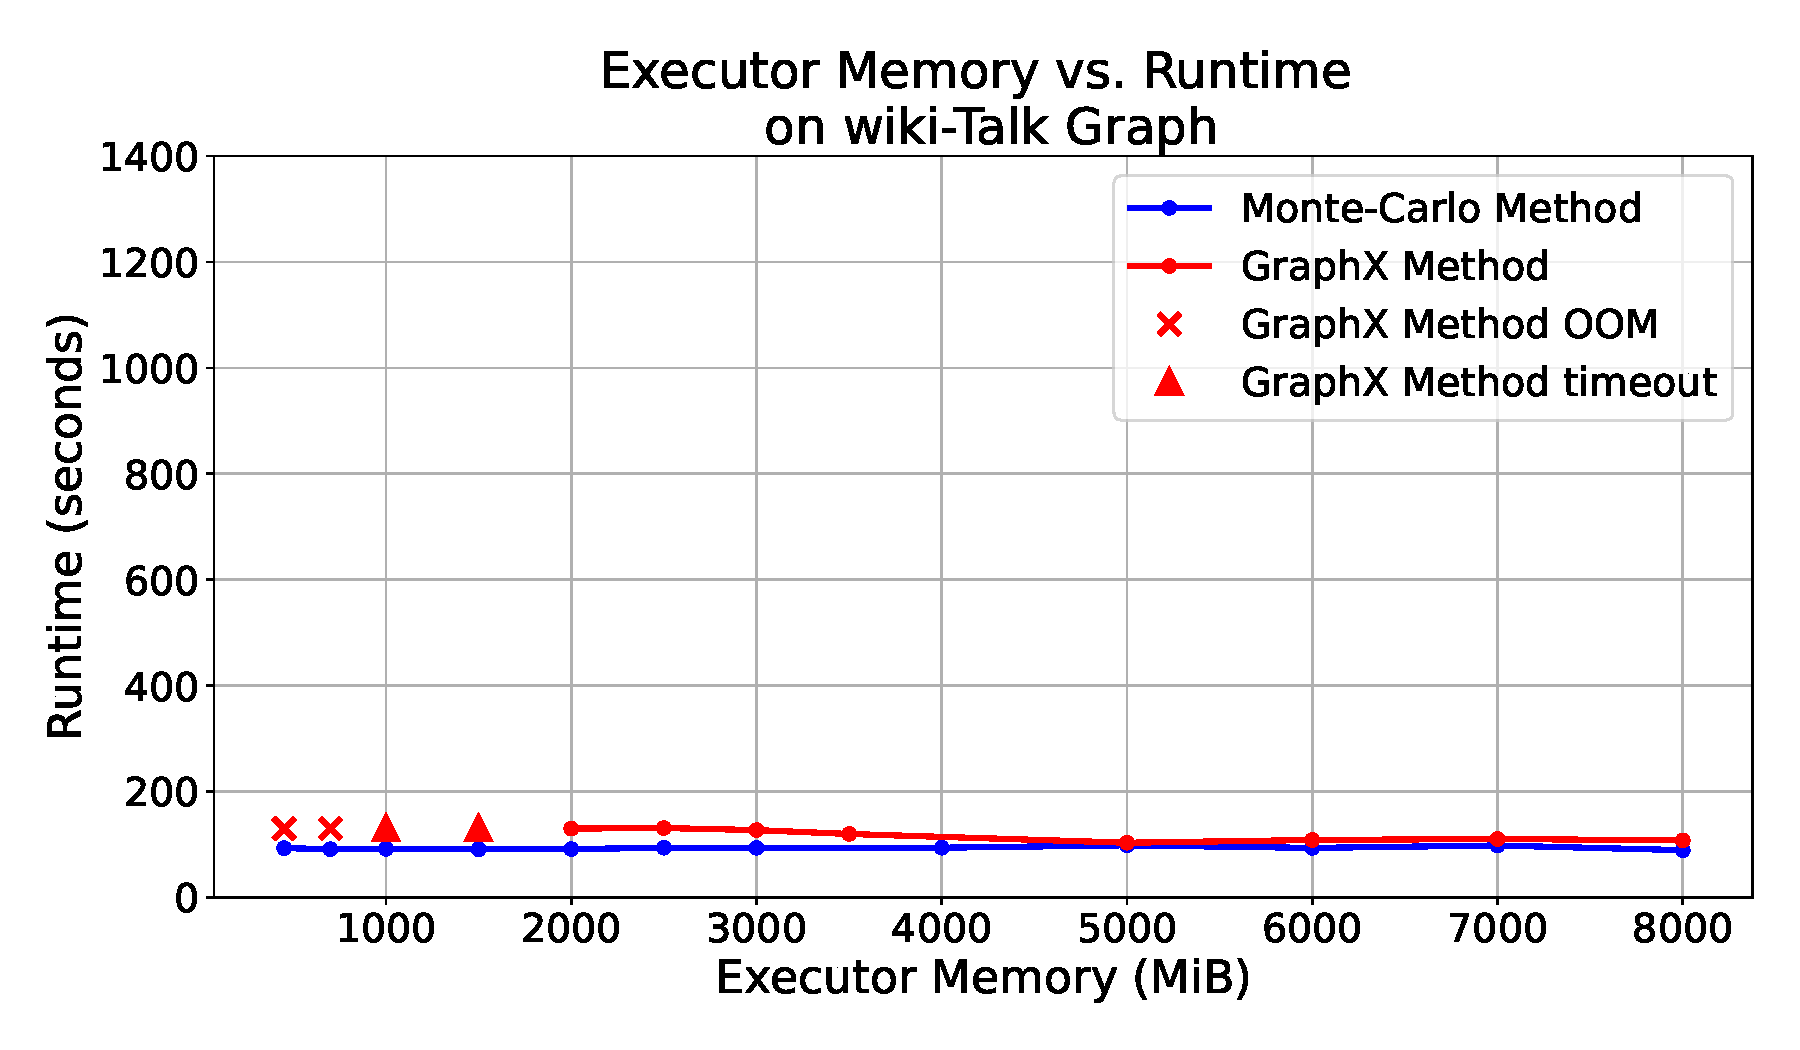
\includegraphics[width=\linewidth]{images/plots/wiki-Talk/memory_vs_runtime_wiki_talk.pdf}
        \caption{Memory vs. Runtime}
        \label{fig:wikirun}
    \end{subfigure}\hfill
    \begin{subfigure}[t]{0.5\linewidth}
        \centering
        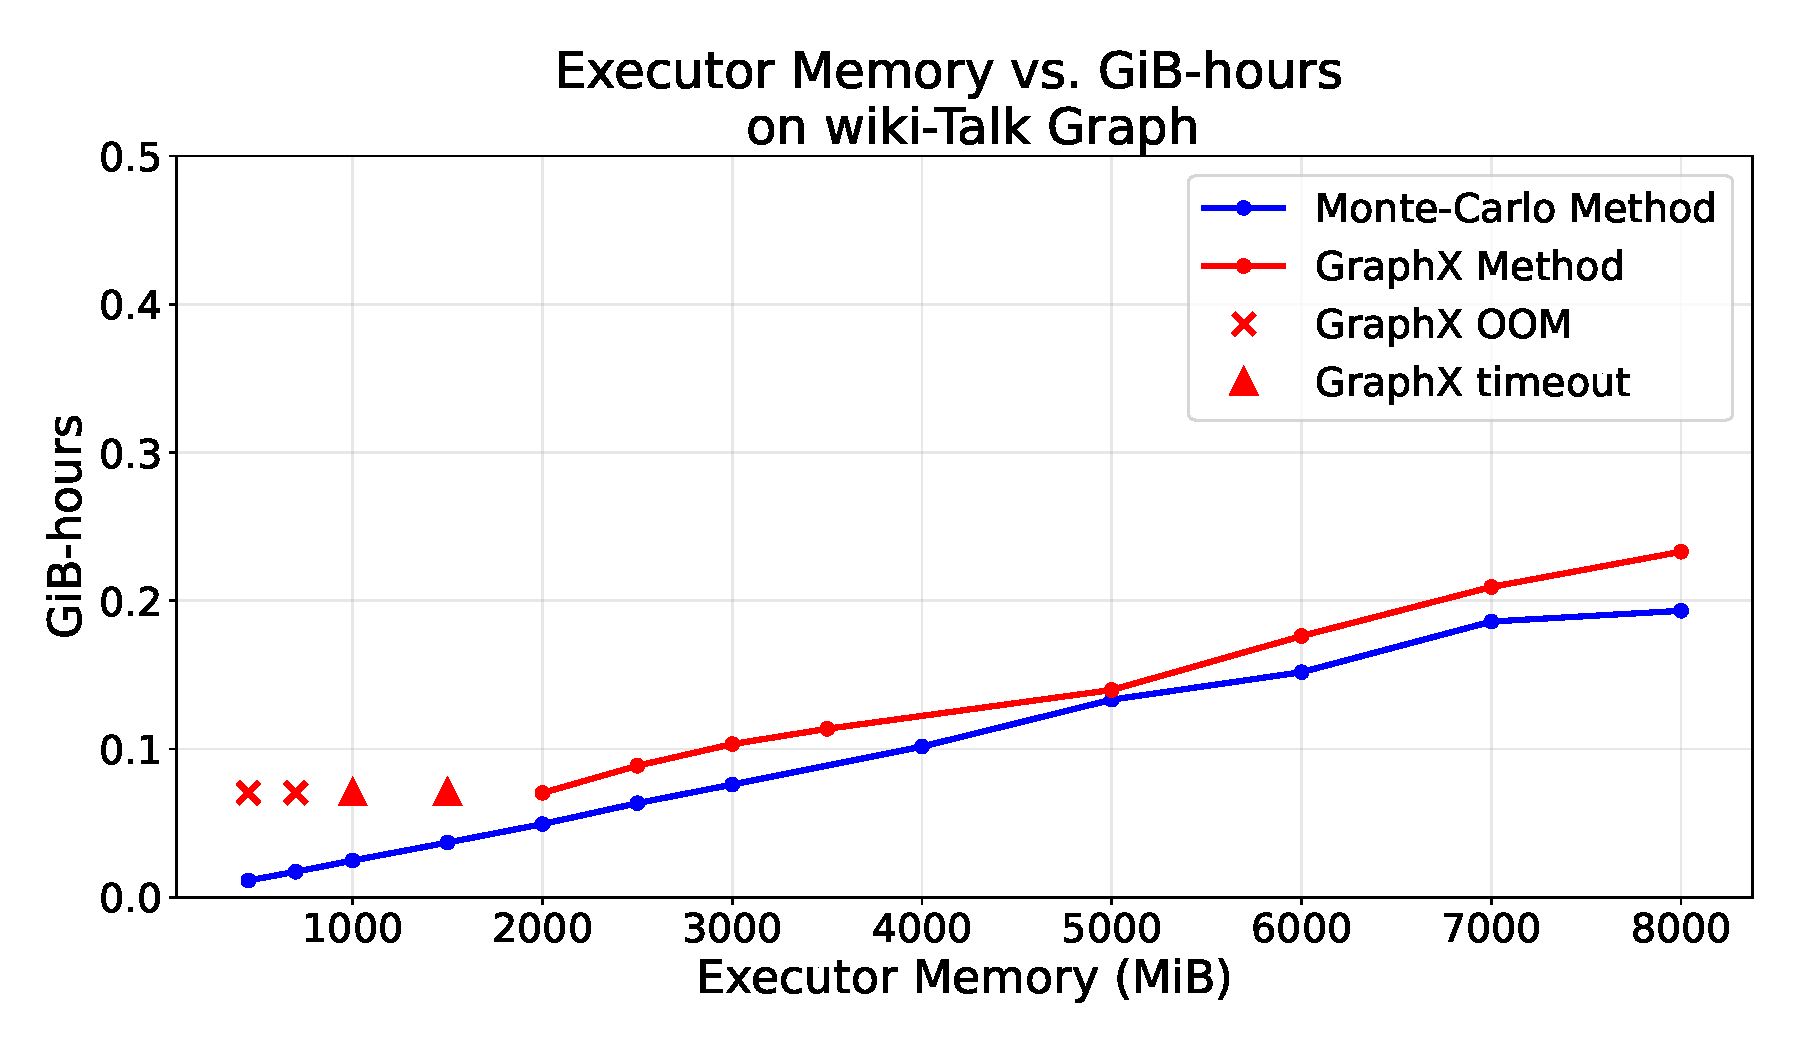
\includegraphics[width=\linewidth]{images/plots/wiki-Talk/gbhrs_nodes_wiki_talk.pdf}
        \caption{GiB-hours}
        \label{fig:wikigibhrs}
    \end{subfigure}
    \begin{subfigure}[t]{0.5\linewidth}
        \centering
        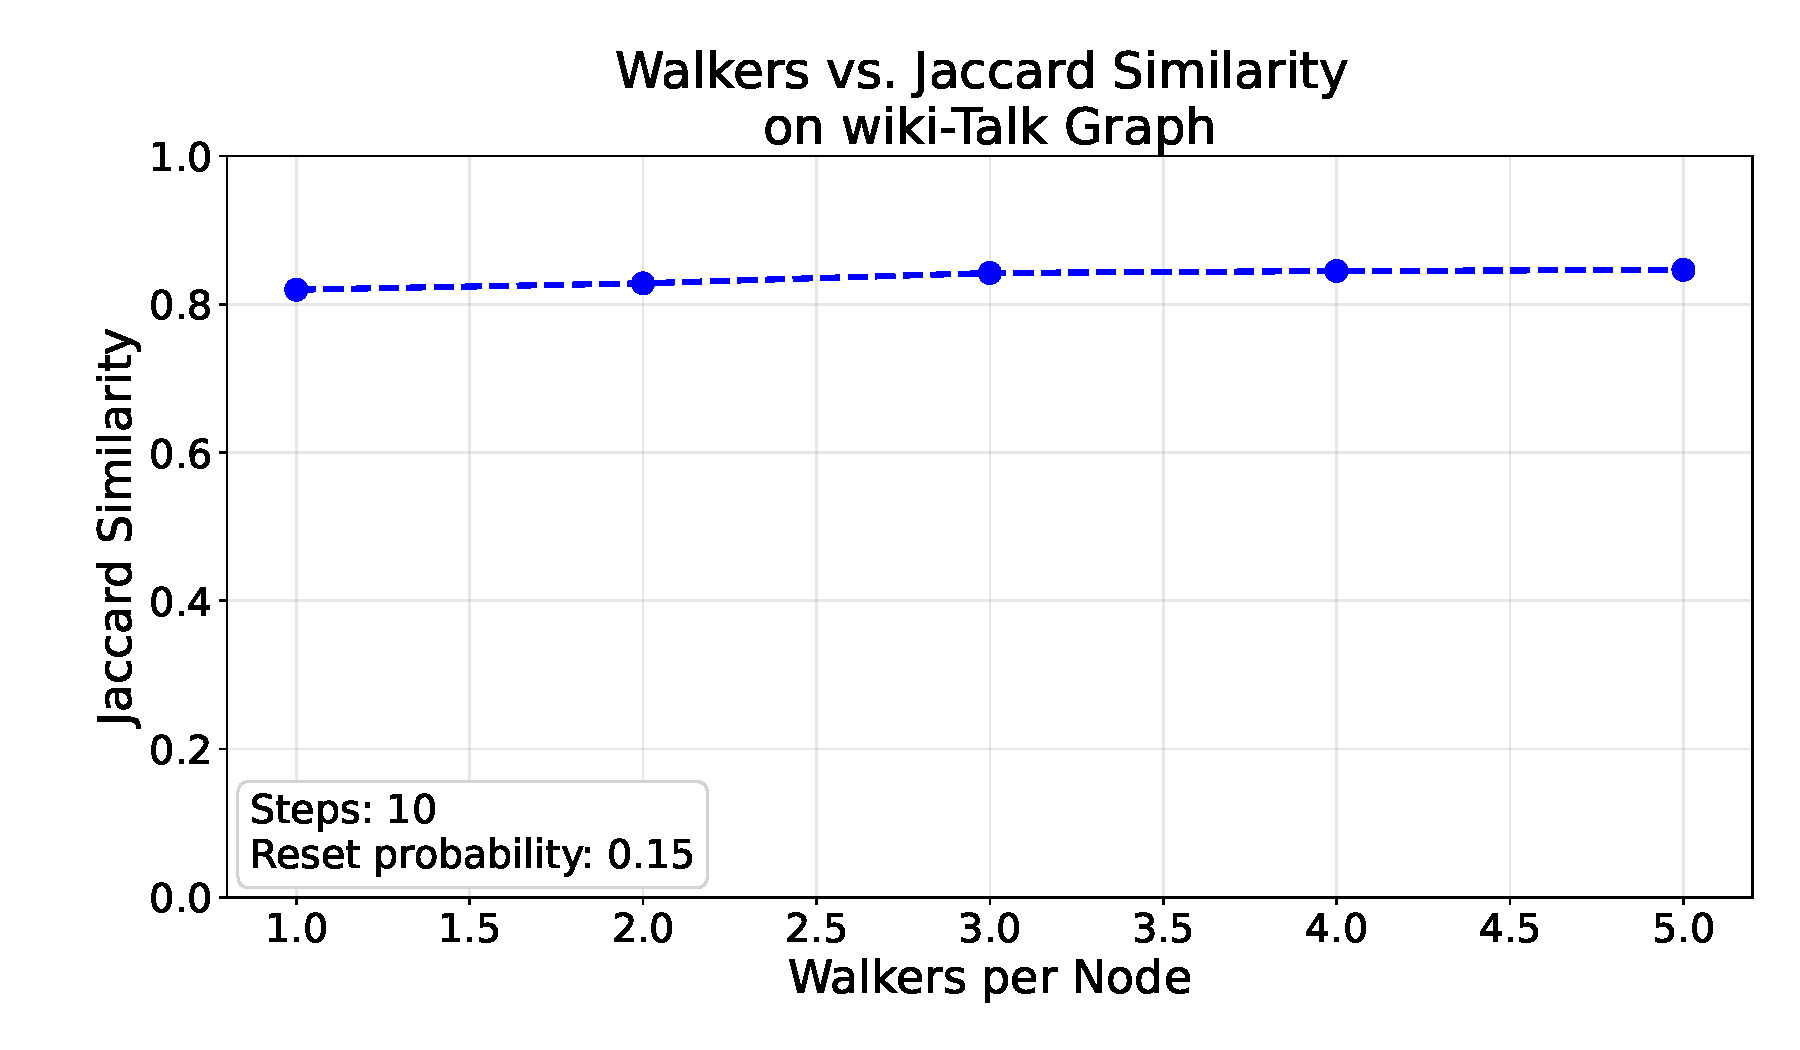
\includegraphics[width=\linewidth]{images/plots/wiki-Talk/accuracy_plots_wiki_talk.pdf}
        \caption{Accuracy}
        \label{fig:wikigibhrs}
    \end{subfigure}
    \caption{PageRank on wiki-Talk Graph}
    \label{fig:wiki-comparison}
\end{figure}

\begin{figure}[H]
    \centering
    \begin{subfigure}[t]{0.5\linewidth}
        \centering
        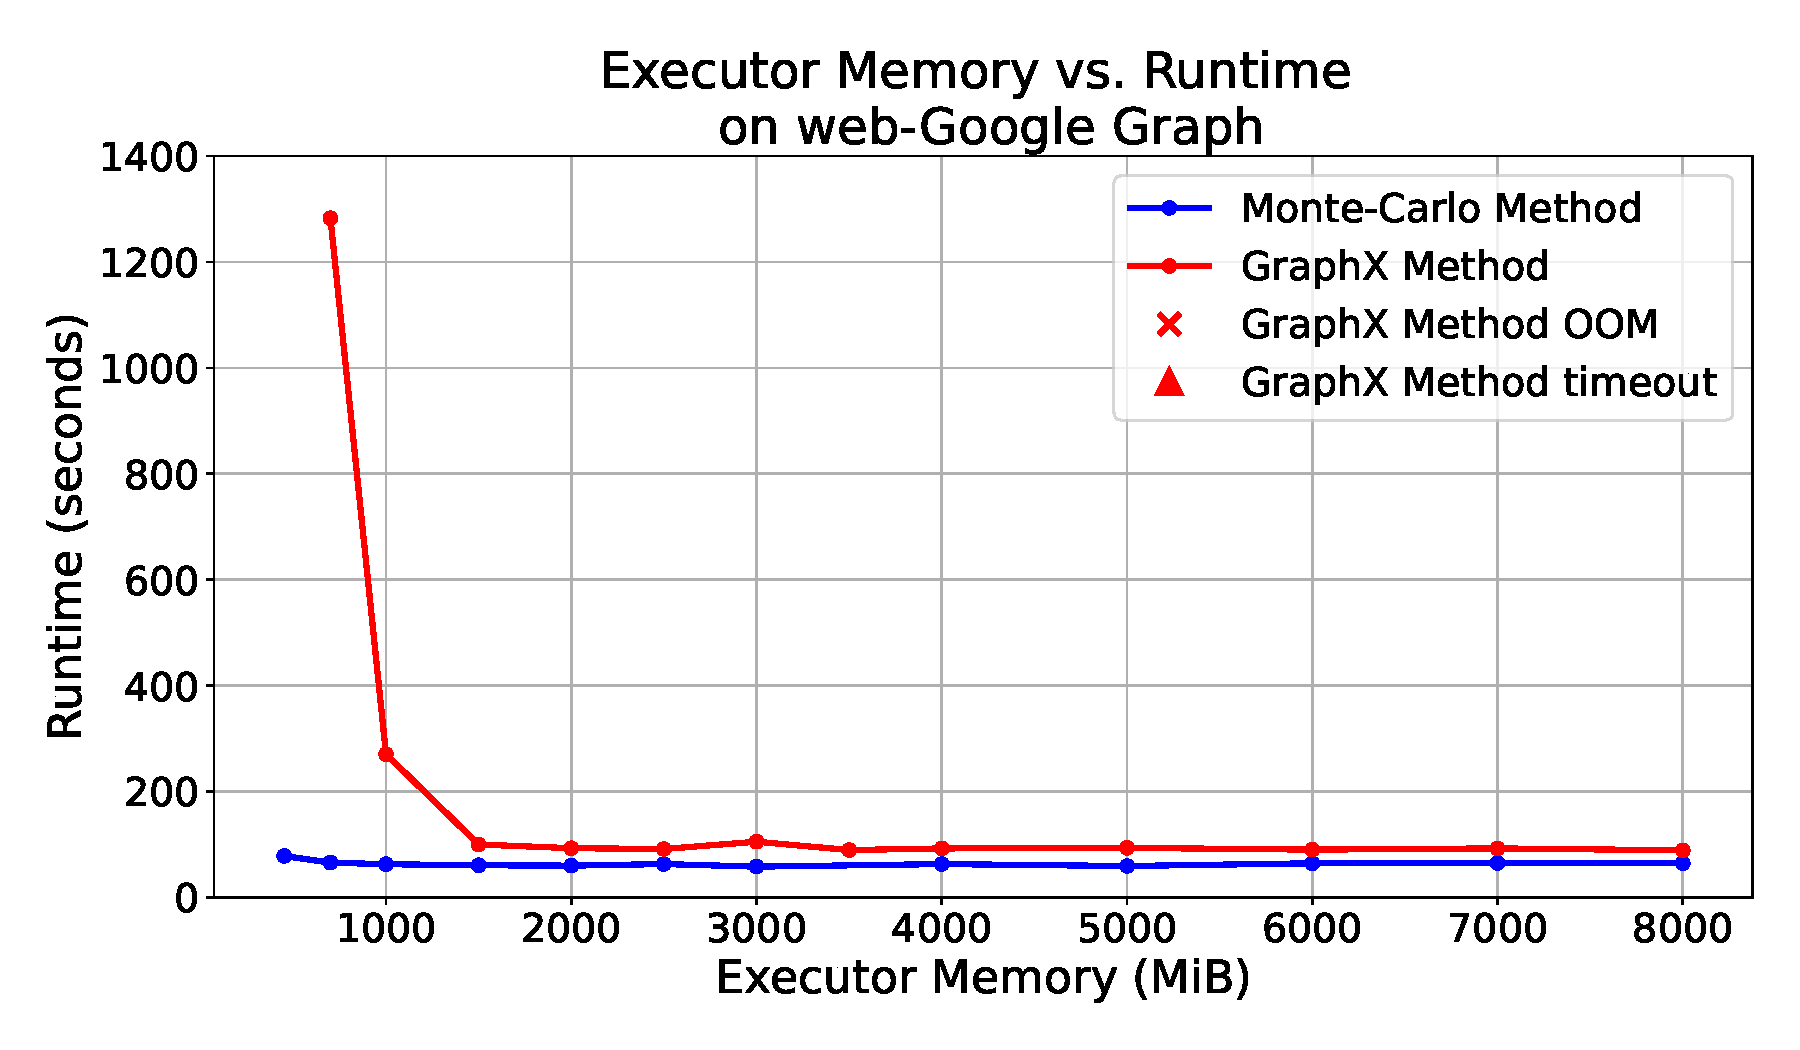
\includegraphics[width=\linewidth]{images/plots/web-Google/memory_vs_runtime_web_google.pdf}
        \caption{Memory vs. Runtime}
        \label{fig:wikirun}
    \end{subfigure}\hfill
    \begin{subfigure}[t]{0.5\linewidth}
        \centering
        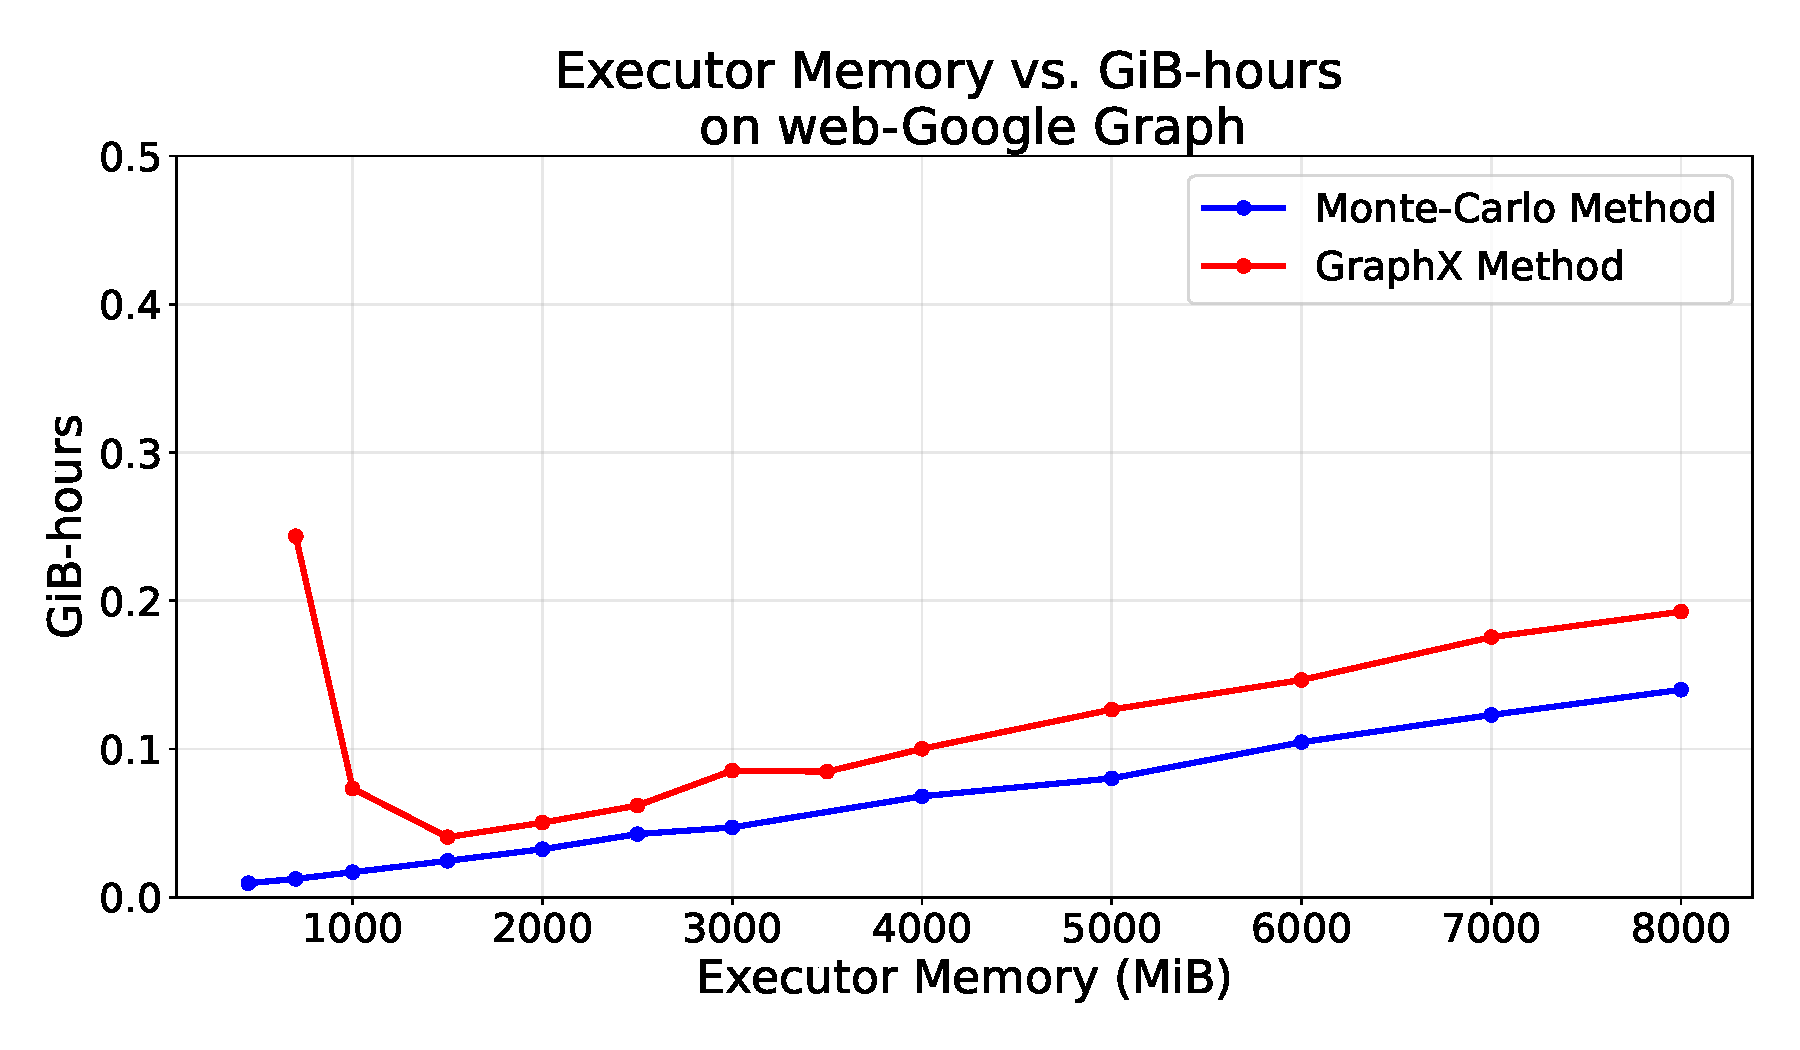
\includegraphics[width=\linewidth]{images/plots/web-Google/gbhrs_nodes_web_google.pdf}
        \caption{GiB-hours}
        \label{fig:wikigibhrs}
    \end{subfigure}
    \begin{subfigure}[t]{0.5\linewidth}
        \centering
        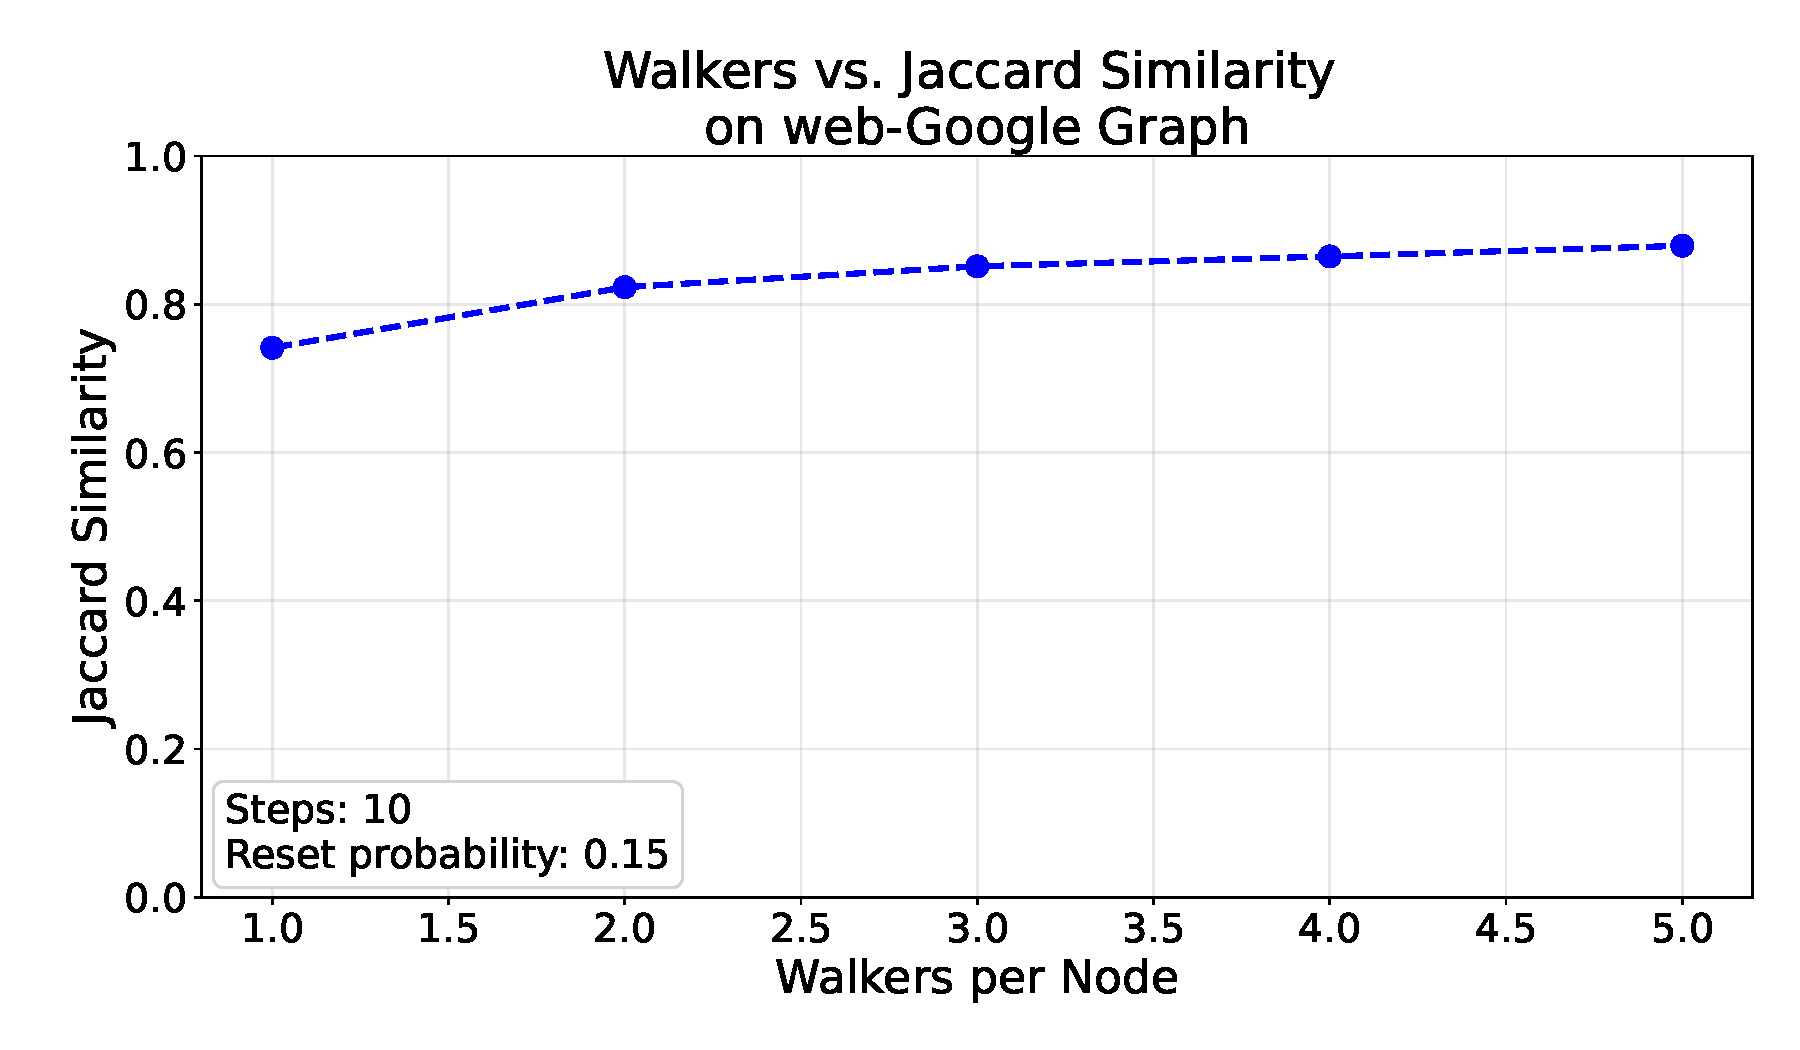
\includegraphics[width=\linewidth]{images/plots/web-Google/accuracy_plots_web_google.pdf}
        \caption{Accuracy}
        \label{fig:wikigibhrs}
    \end{subfigure}
    \caption{PageRank on web-Google Graph}
    \label{fig:wiki-comparison}
\end{figure}

% \begin{figure}[H]
%     \centering
%     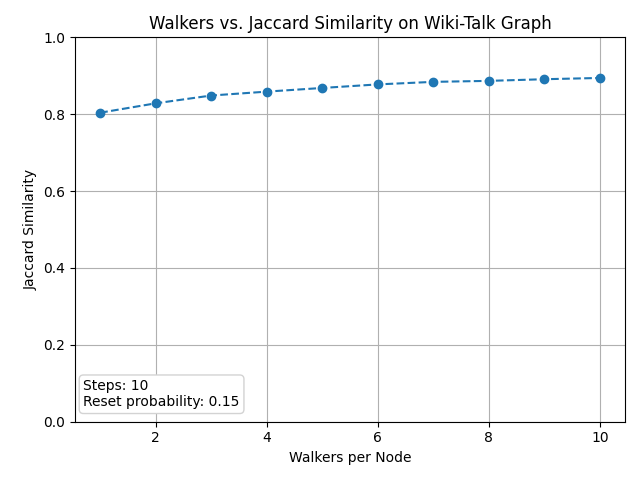
\includegraphics[width=\linewidth]{images/plots/wiki-Talk/steps_vs_accuracy_server_edited.png}
%     \caption{Accuracy}
%     \label{fig:wikiacc}
% \end{figure}

\begin{figure}[H]
    \centering
    \begin{subfigure}[t]{0.75\linewidth}
        \centering
        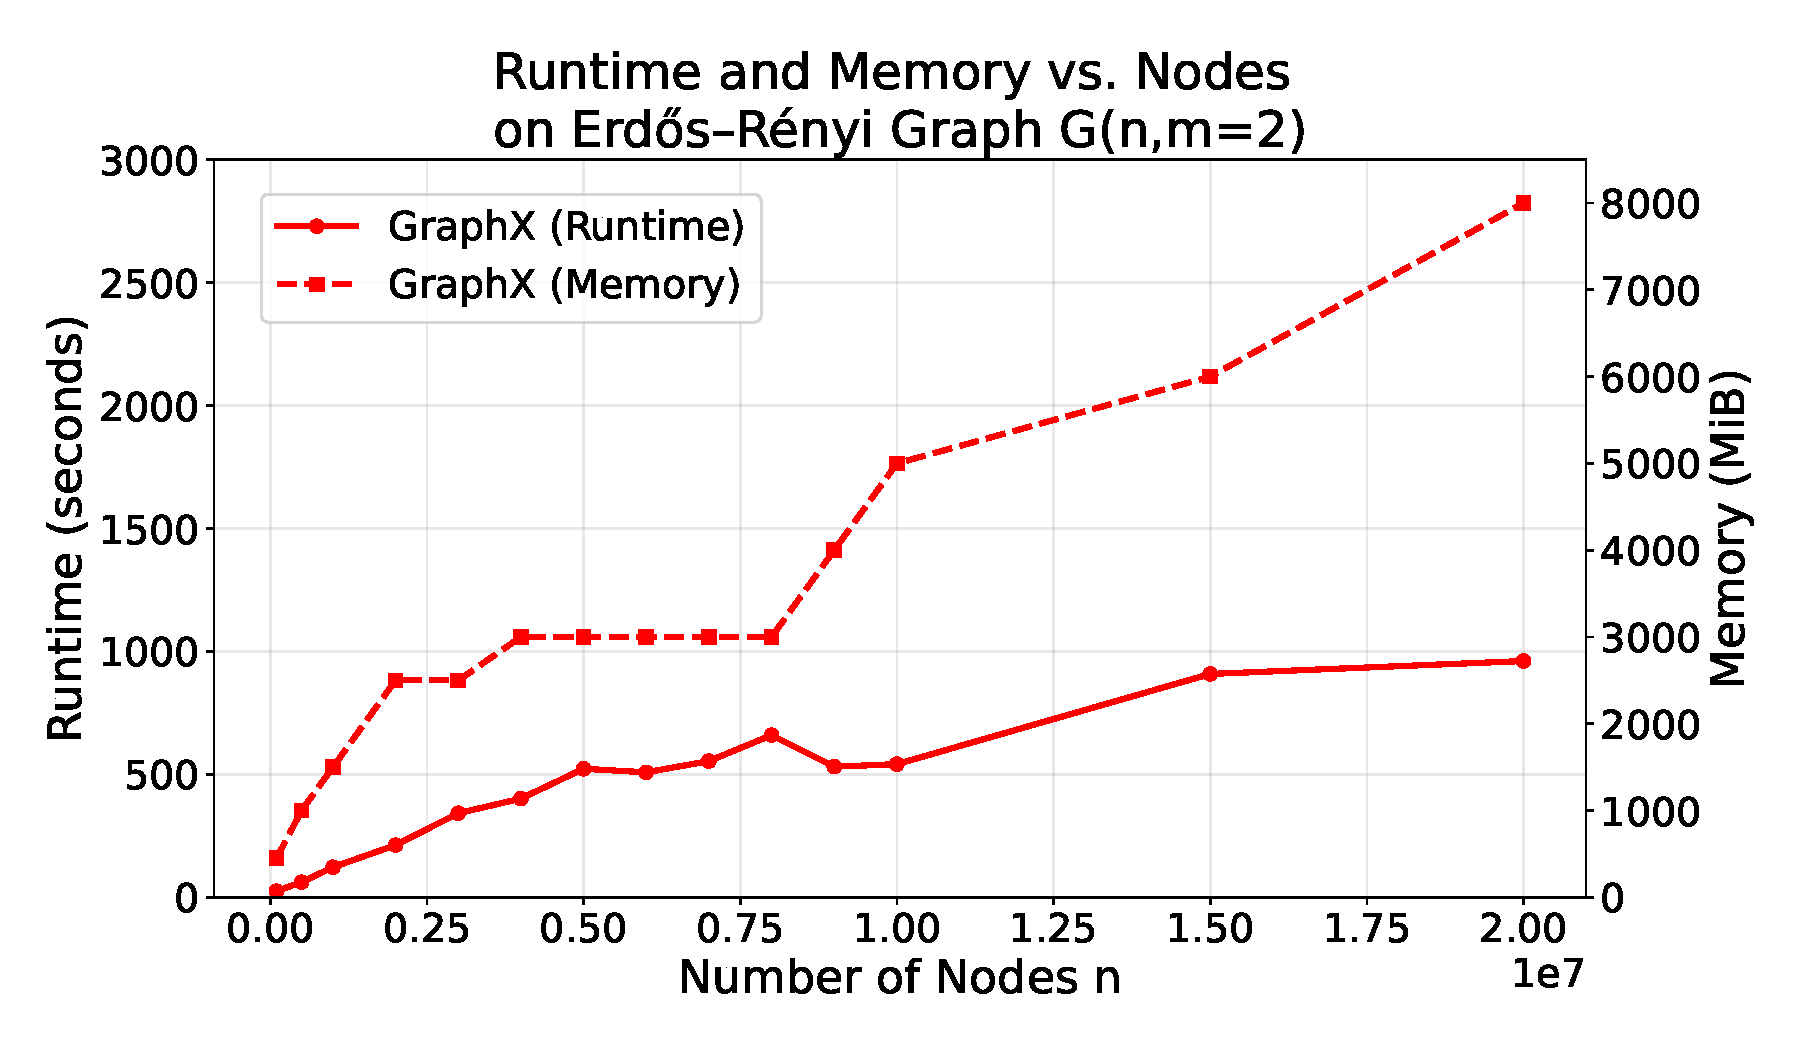
\includegraphics[width=\linewidth]{images/plots/ER_2edg/combined_runtime_memory_vs_nodes_2edges_v3.pdf}
        \caption{2 edges per node}
        \label{fig:2run}
    \end{subfigure}\hfill
    \begin{subfigure}[t]{0.75\linewidth}
        \centering
        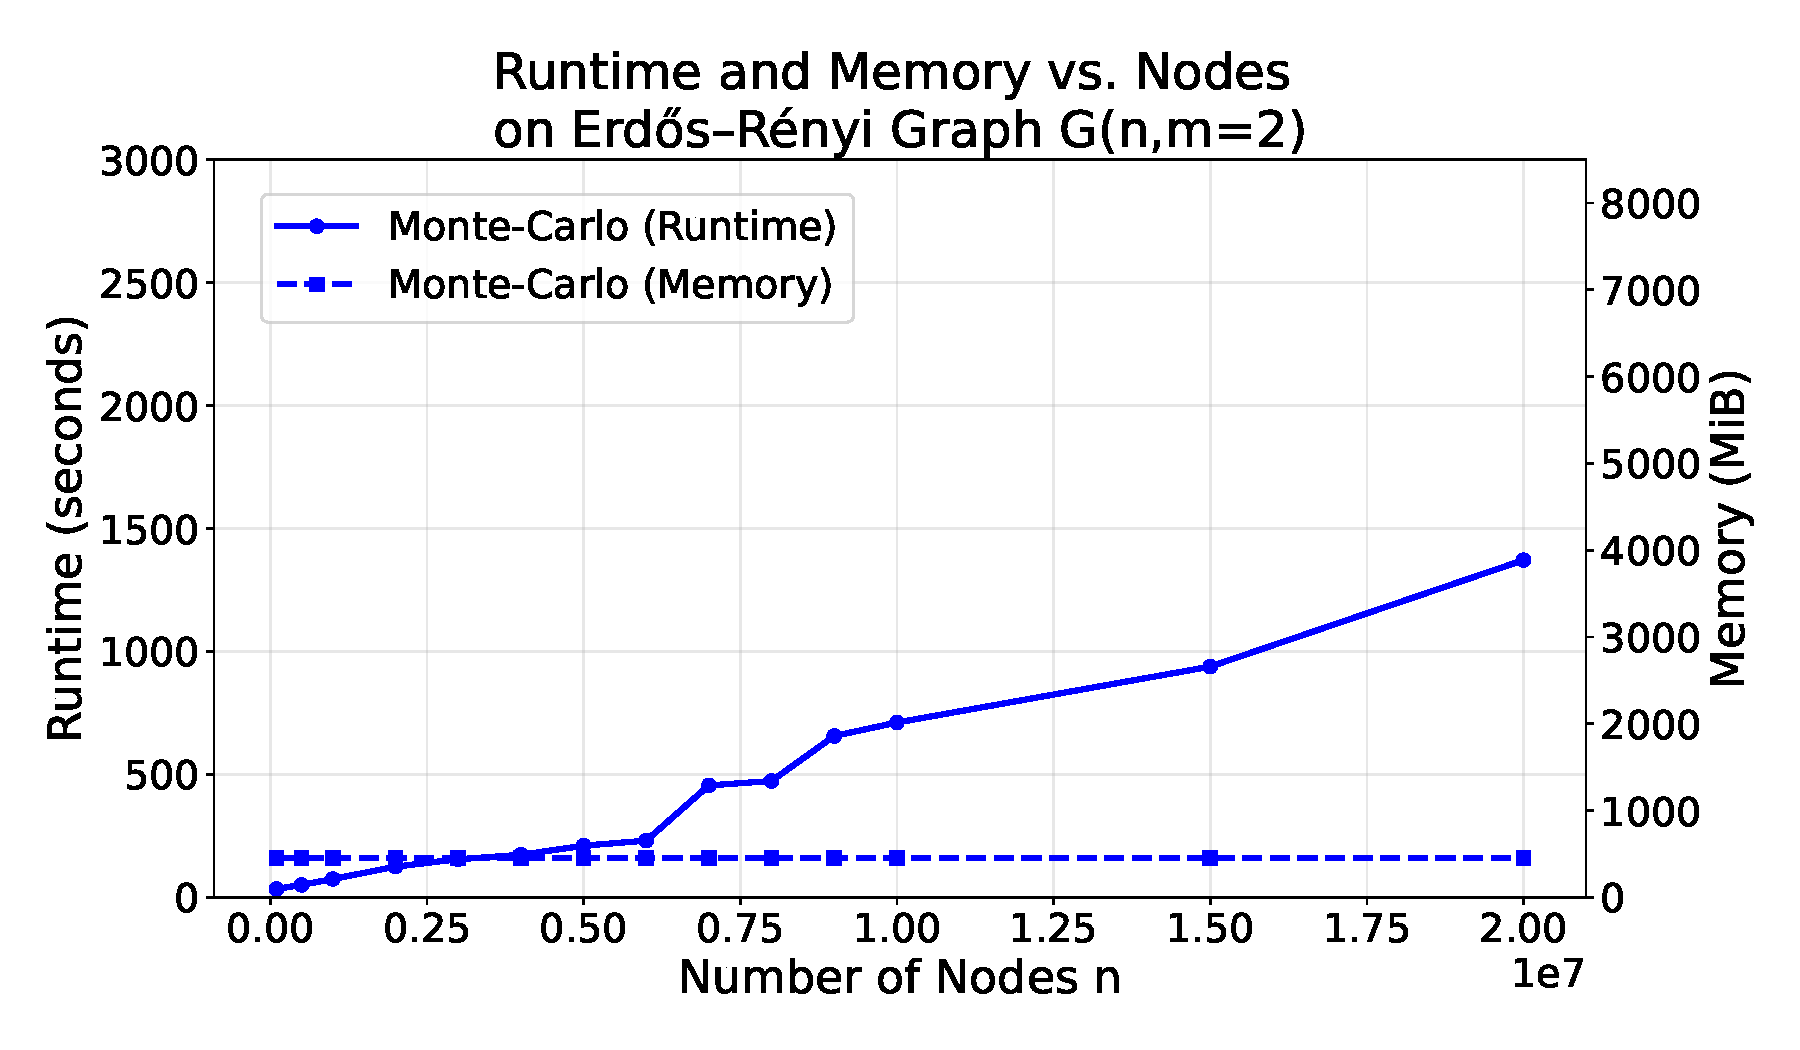
\includegraphics[width=\linewidth]{images/plots/ER_2edg/combined_runtime_memory_vs_nodes_2edges_mc.pdf}
        \caption{2 edges per node}
        \label{fig:2cost}
    \end{subfigure}
    \begin{subfigure}[t]{0.75\linewidth}
        \centering
        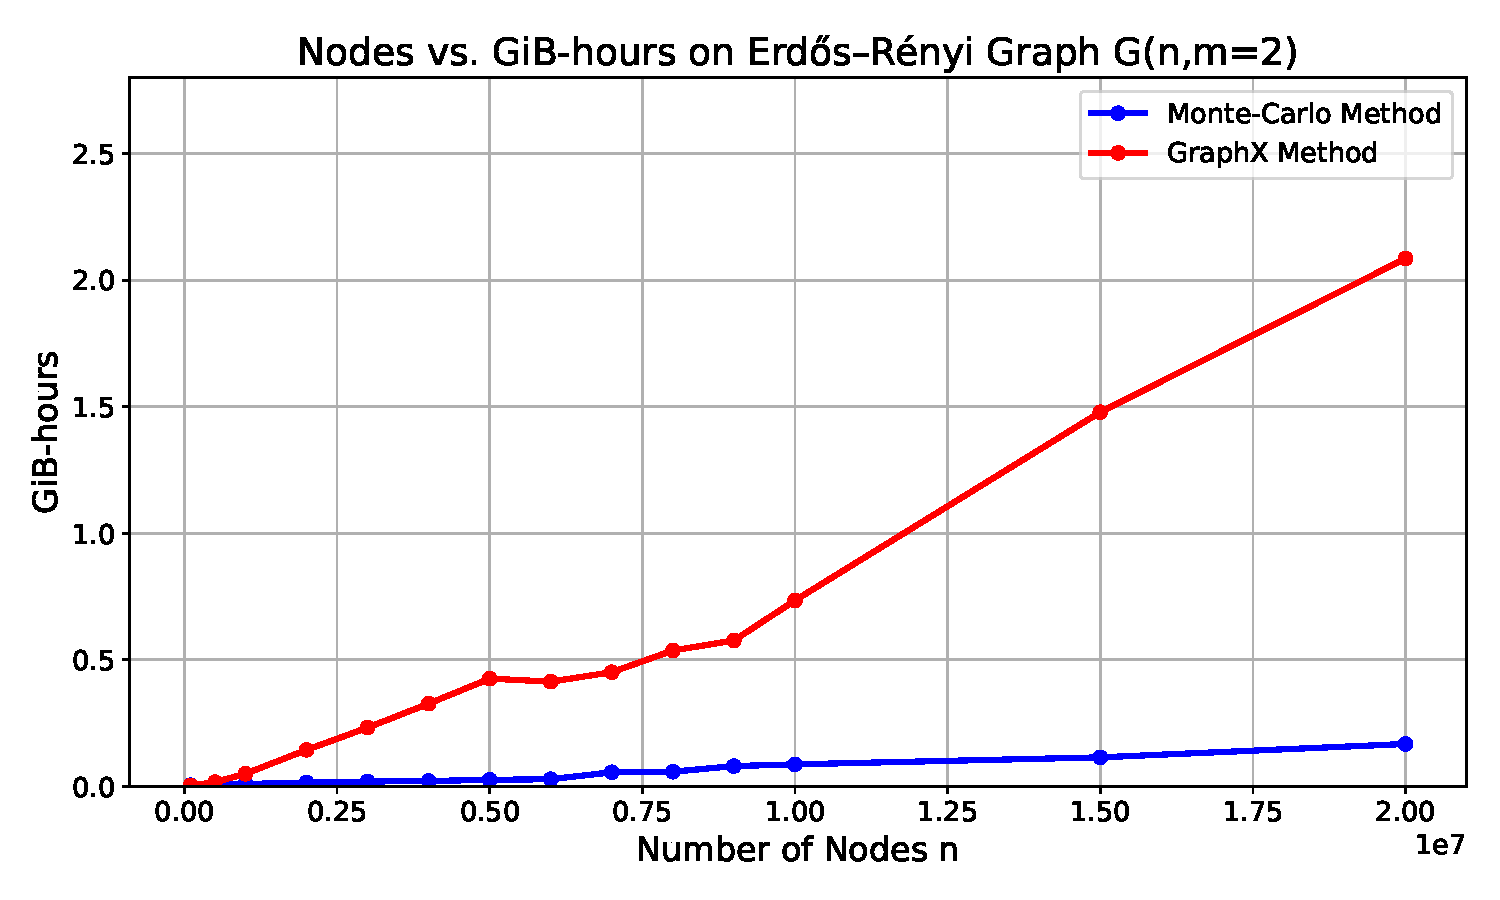
\includegraphics[width=\linewidth]{images/plots/ER_2edg/gbhrs_nodes_er_graph_2edges.pdf}
        \caption{2 edges per node}
        \label{fig:2cost}
    \end{subfigure}
\end{figure}



\begin{figure}[H]
    \centering
    \begin{subfigure}[t]{0.75\linewidth}
        \centering
        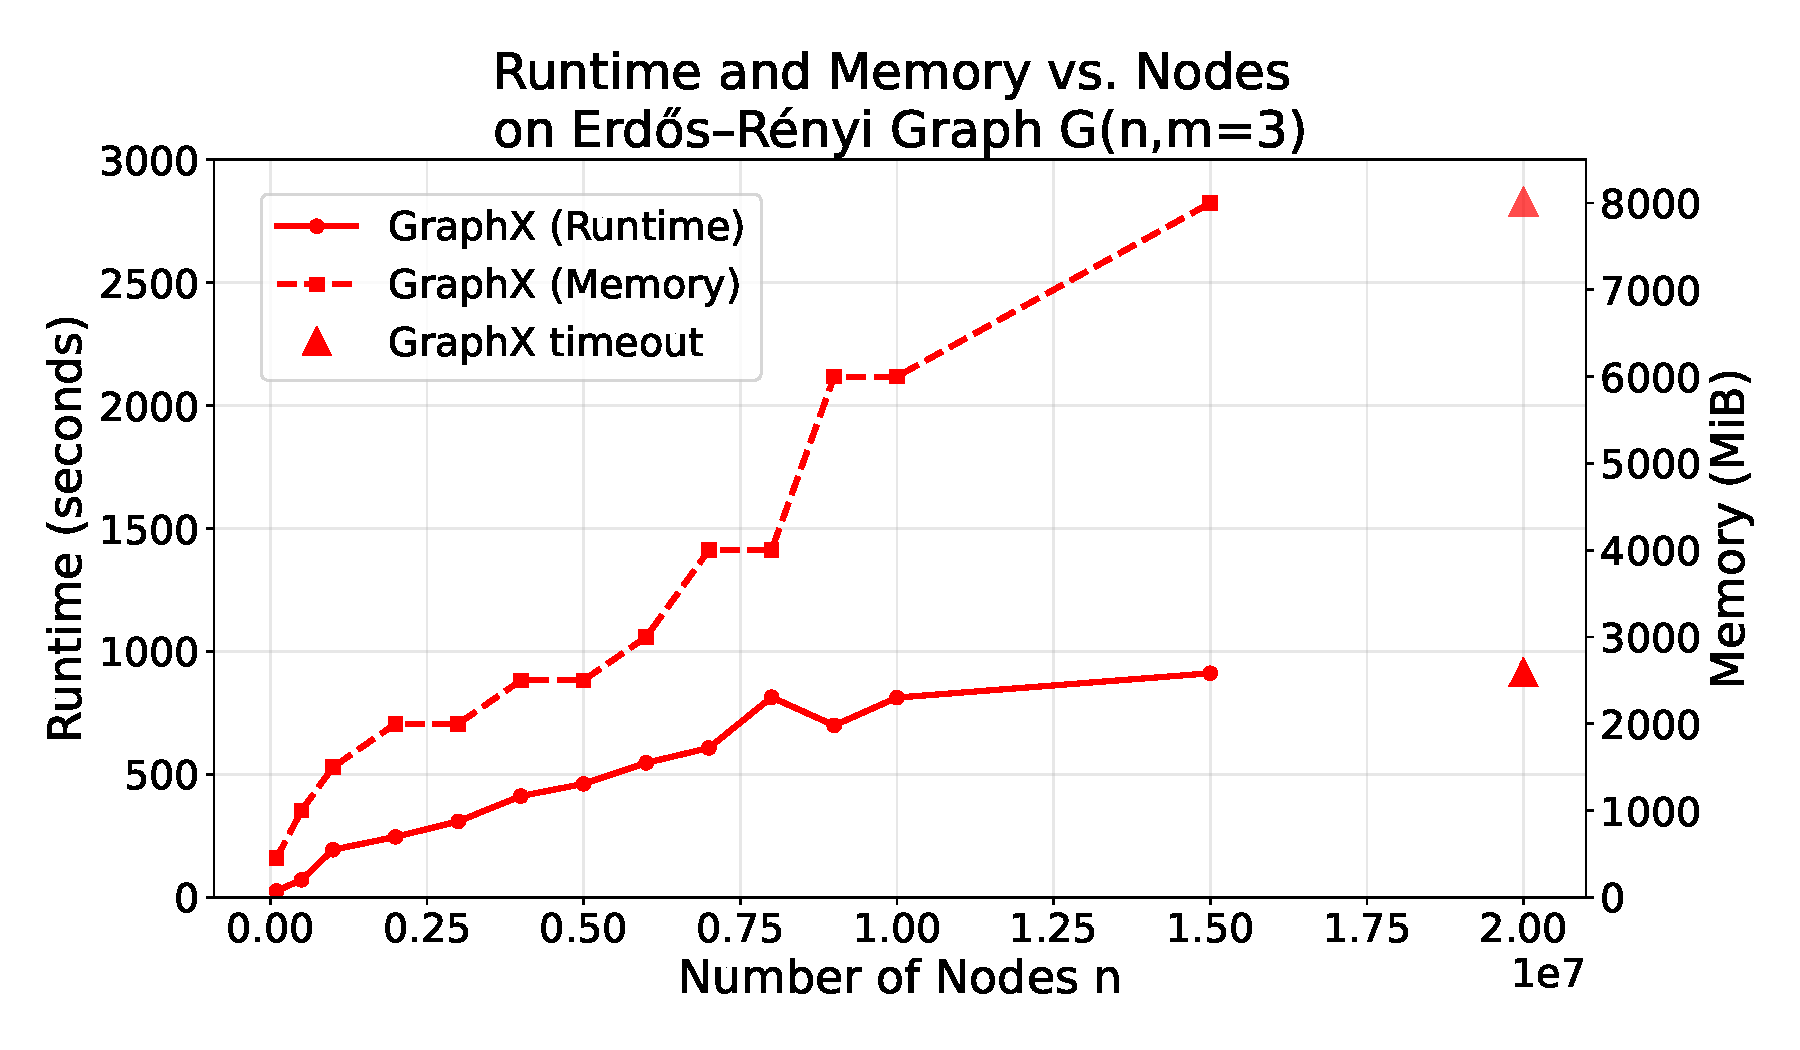
\includegraphics[width=\linewidth]{images/plots/ER_3edg/combined_runtime_memory_vs_nodes_3edges_gx.pdf}
        \caption{3 edges per node}
        \label{fig:3run}
    \end{subfigure}
    \begin{subfigure}[t]{0.75\linewidth}
        \centering
        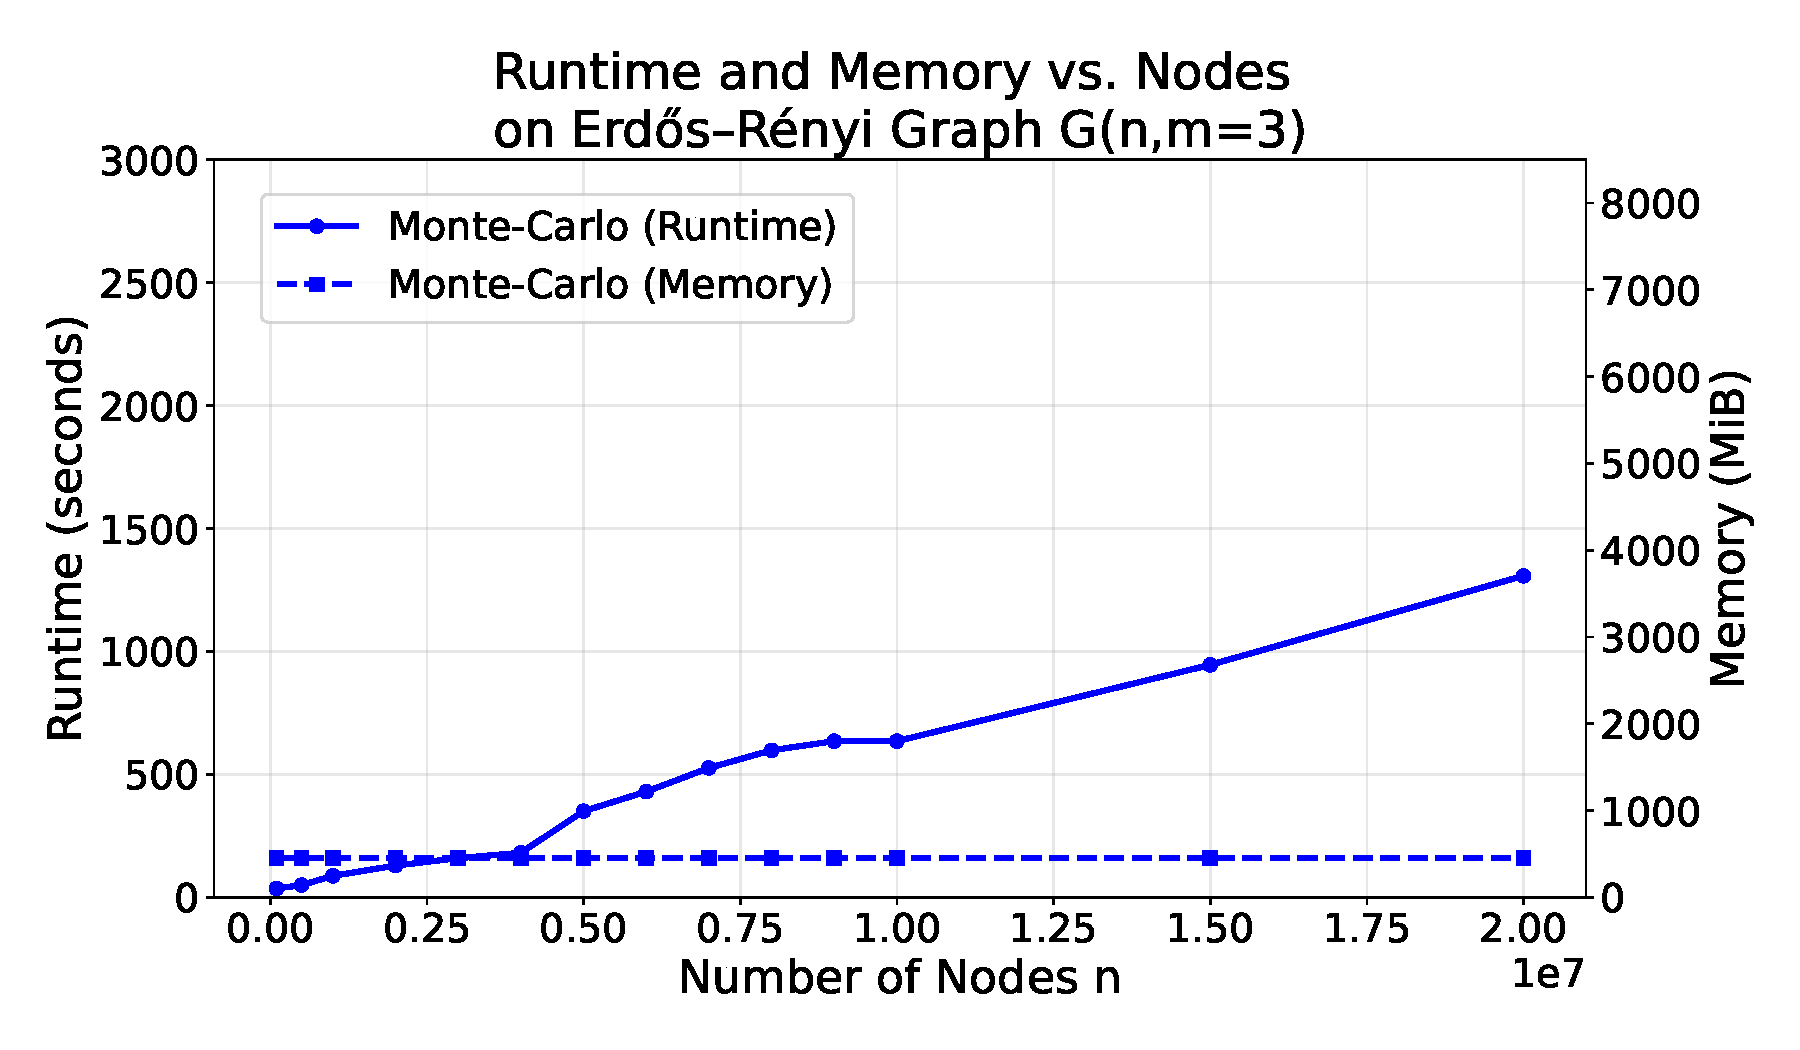
\includegraphics[width=\linewidth]{images/plots/ER_3edg/combined_runtime_memory_vs_nodes_3edges_mc.pdf}
        \caption{3 edges per node}
        \label{fig:3cost}
    \end{subfigure}
    \begin{subfigure}[t]{0.75\linewidth}
        \centering
        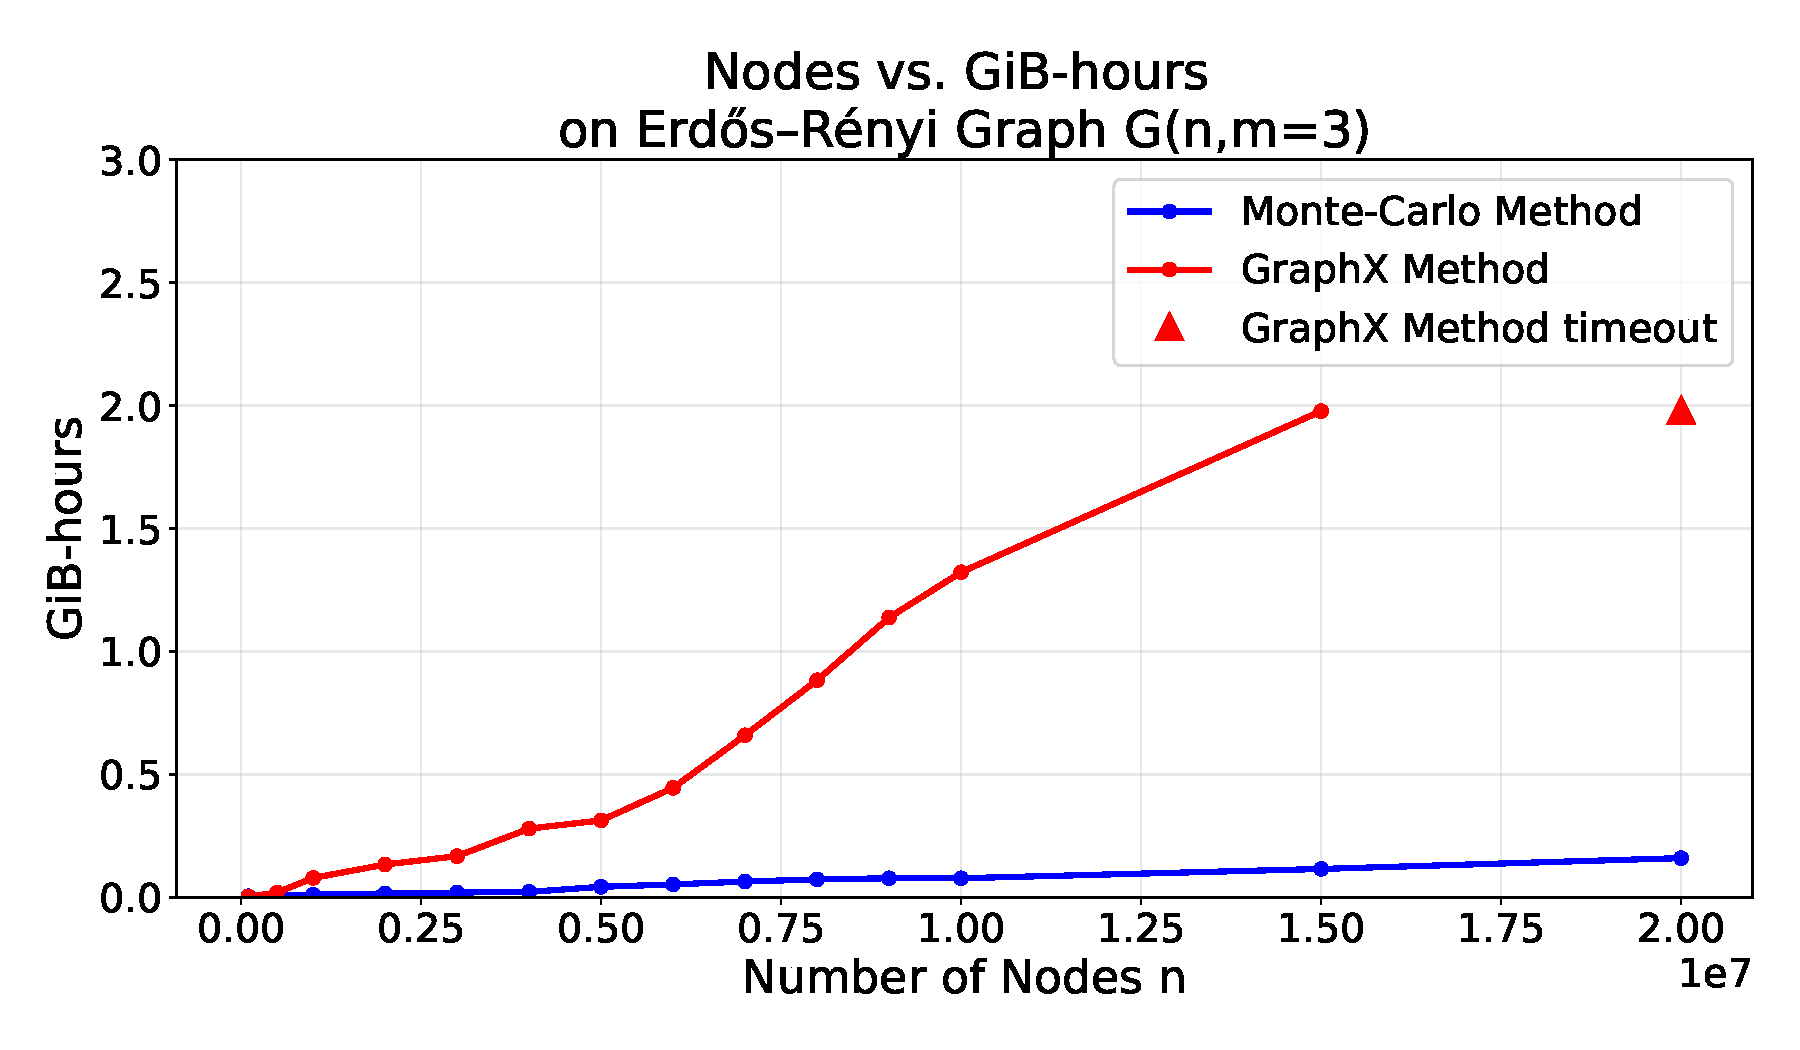
\includegraphics[width=\linewidth]{images/plots/ER_3edg/gbhrs_nodes_er_graph_3edges.pdf}
        \caption{3 edges per node}
        \label{fig:3mvm}
    \end{subfigure}
\end{figure}

% \begin{figure}[H]
%     \centering
%     \begin{subfigure}[t]{0.47\linewidth}
%         \centering
%         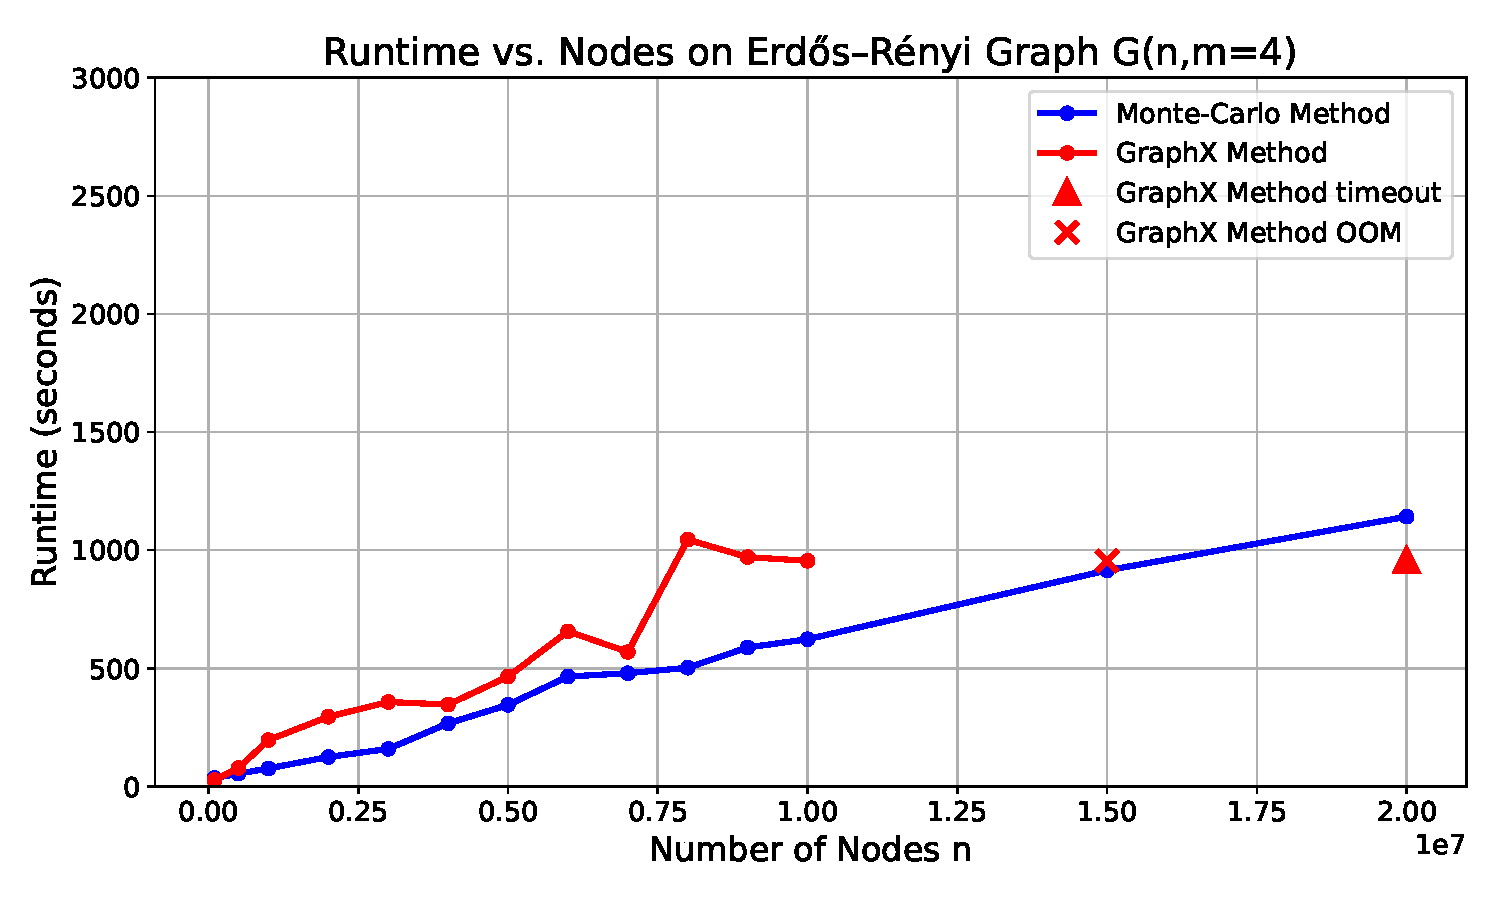
\includegraphics[width=\linewidth]{images/plots/ER_4edg/runtime_vs_nodes_er_graph_4_edges.pdf}
%         \caption{4 edges per node}
%         \label{fig:4run}
%     \end{subfigure}
%     \begin{subfigure}[t]{0.47\linewidth}
%         \centering
%     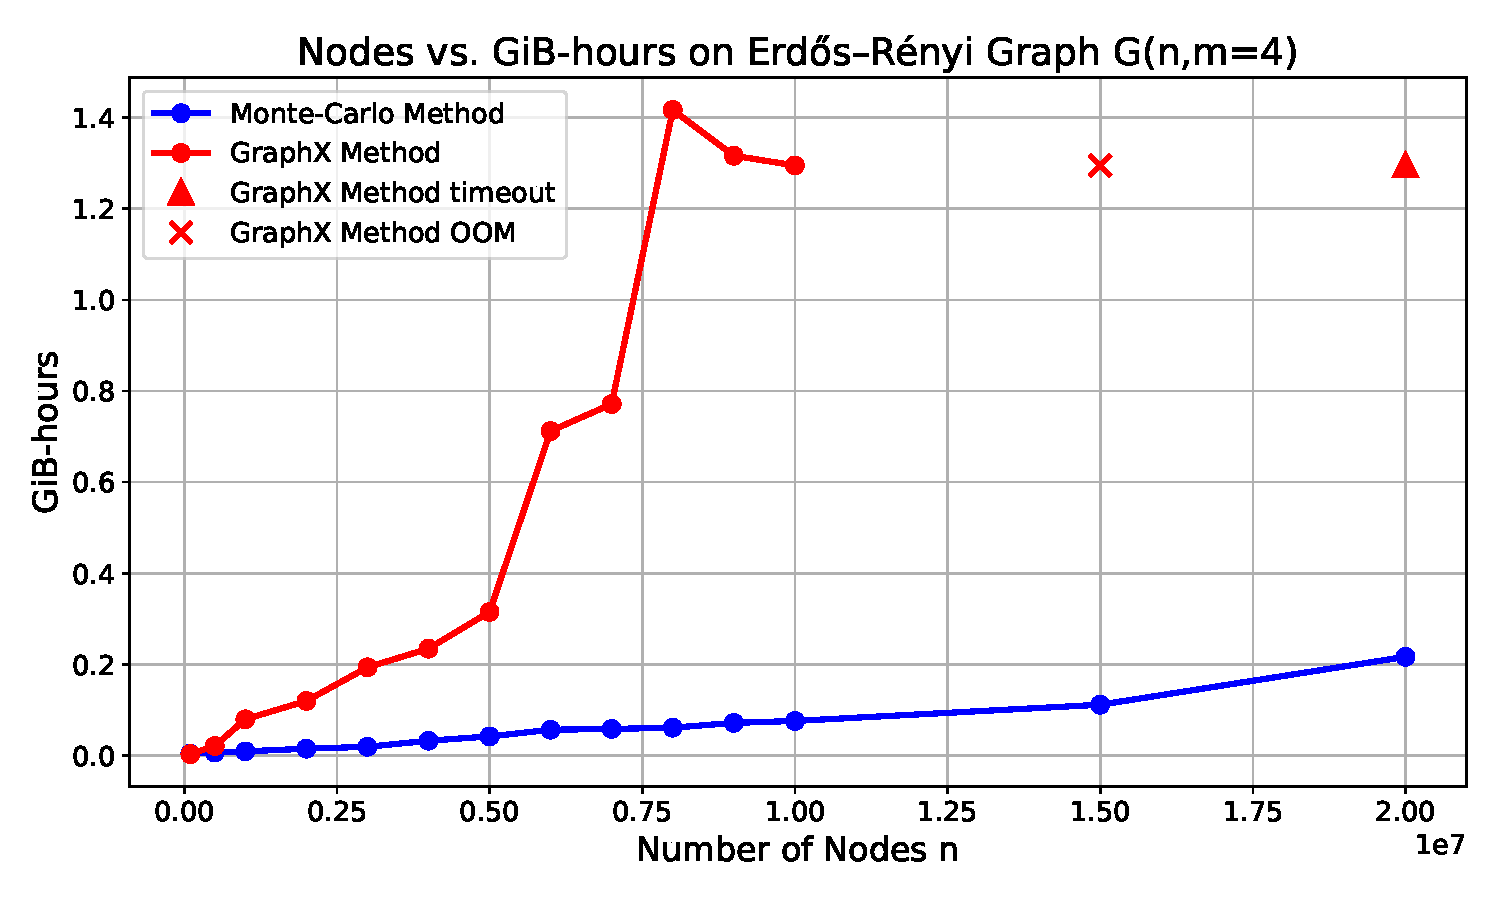
\includegraphics[width=\linewidth]{images/plots/ER_4edg/gbhrs_nodes_er_graph_4edges.pdf}
%         \caption{4 edges per node}
%         \label{fig:4cost}
%     \end{subfigure}
%     \begin{subfigure}[t]{0.47\linewidth}
%         \centering
%         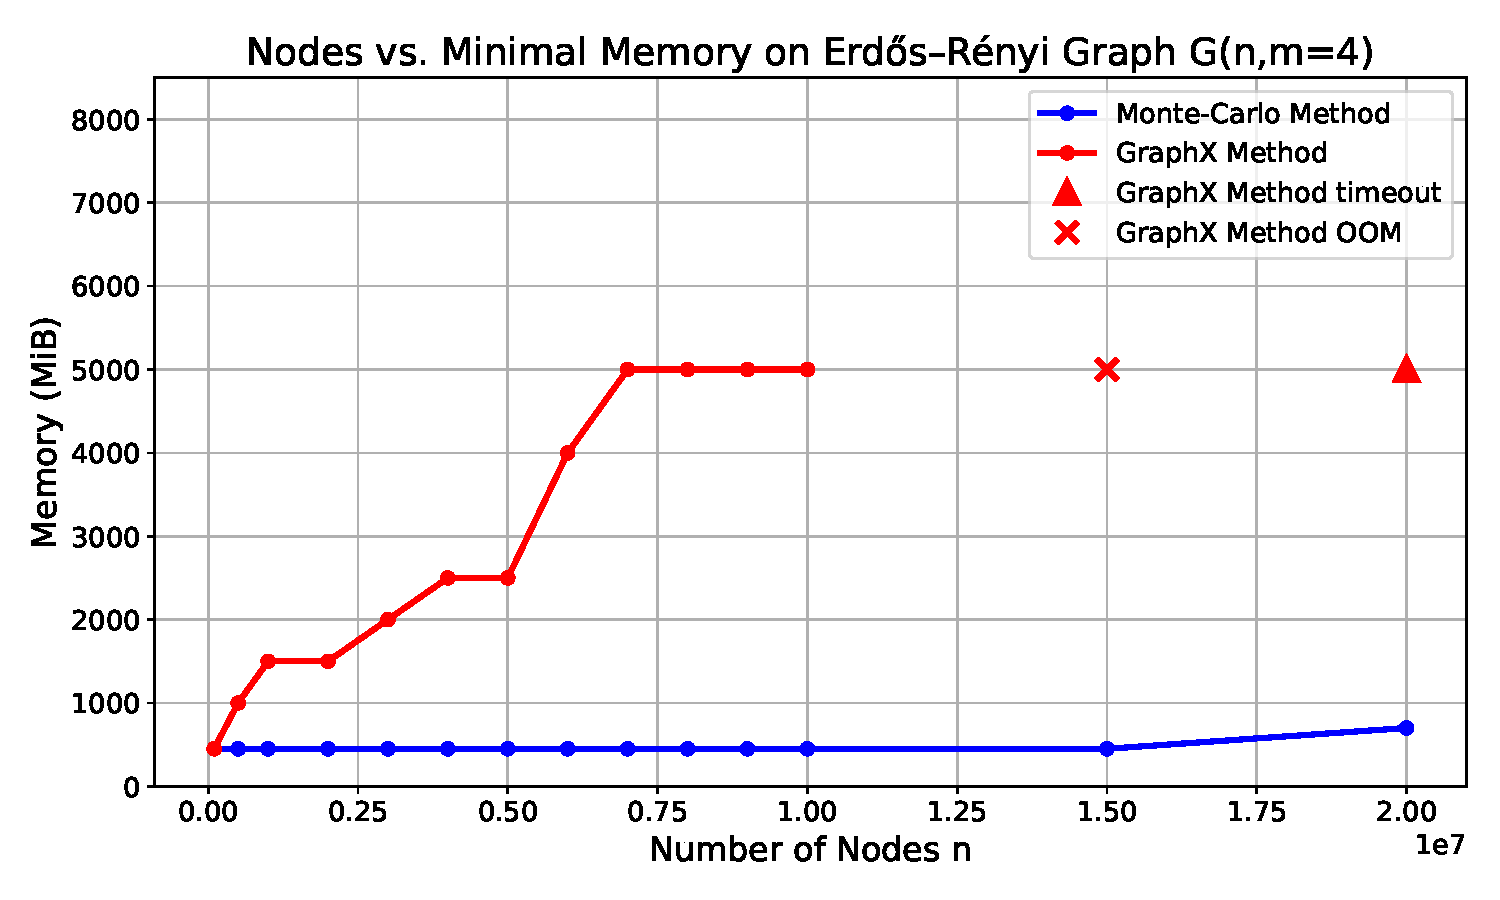
\includegraphics[width=\linewidth]{images/plots/ER_4edg/nodes_vs_mvm_4edges.pdf}
%         \caption{4 edges per node}
%         \label{fig:4run}
%     \end{subfigure}
%     \caption{3 walkers per node and 10 steps per walker}
% \end{figure}

% \begin{figure}[H]
%     \centering
%     \begin{subfigure}[t]{0.47\linewidth}
%         \centering
%         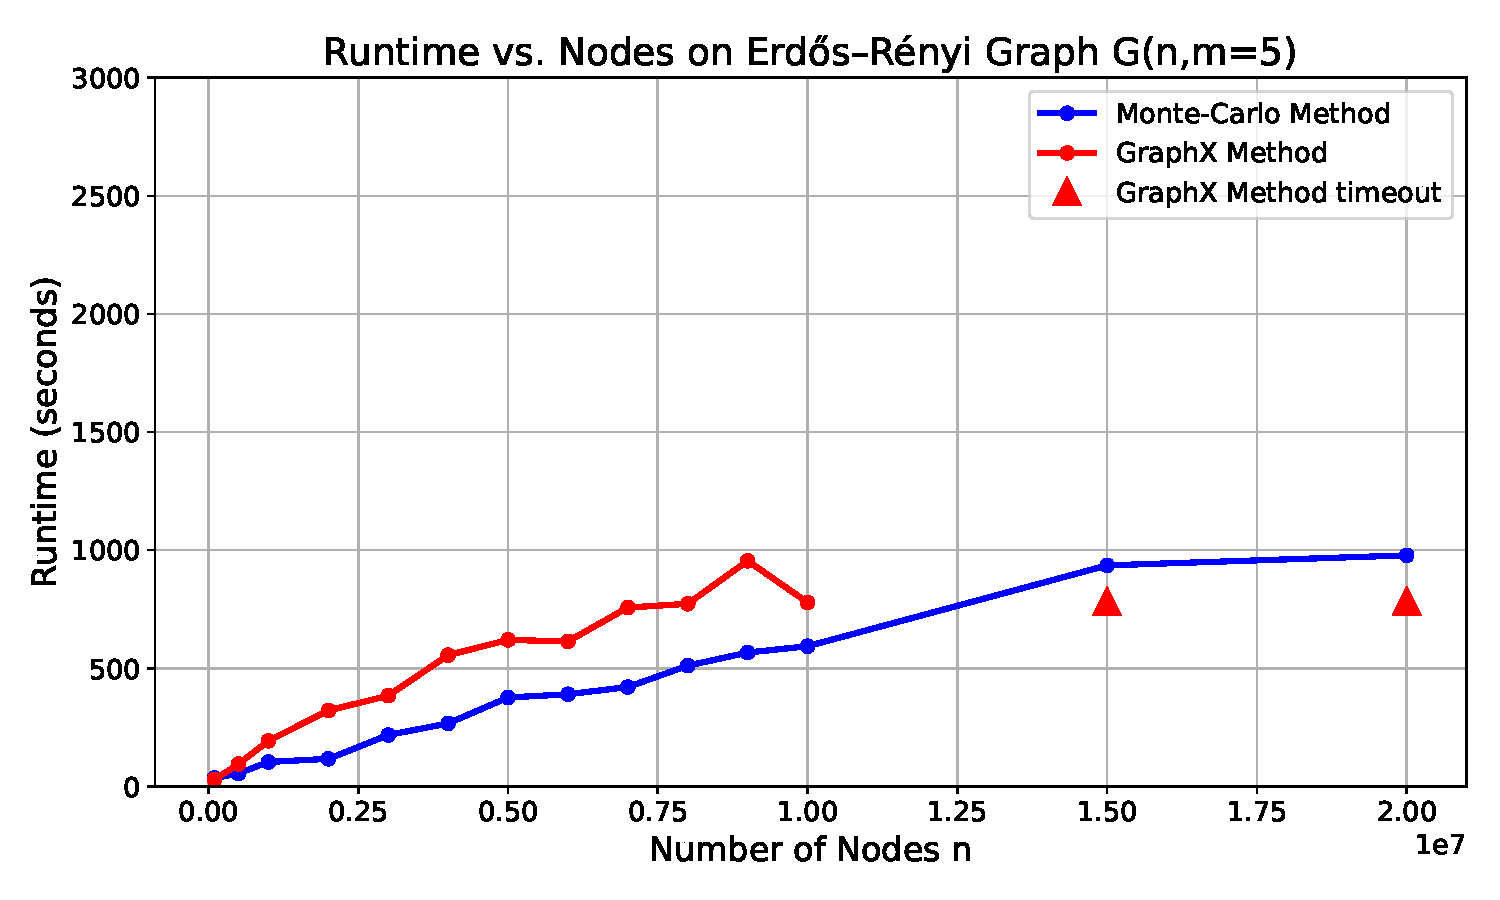
\includegraphics[width=\linewidth]{images/plots/ER_5edg/runtime_vs_nodes_er_graph_5_edges.pdf}
%         \caption{5 edges per node}
%         \label{fig:5run}
%     \end{subfigure}
%     \begin{subfigure}[t]{0.47\linewidth}
%         \centering
%         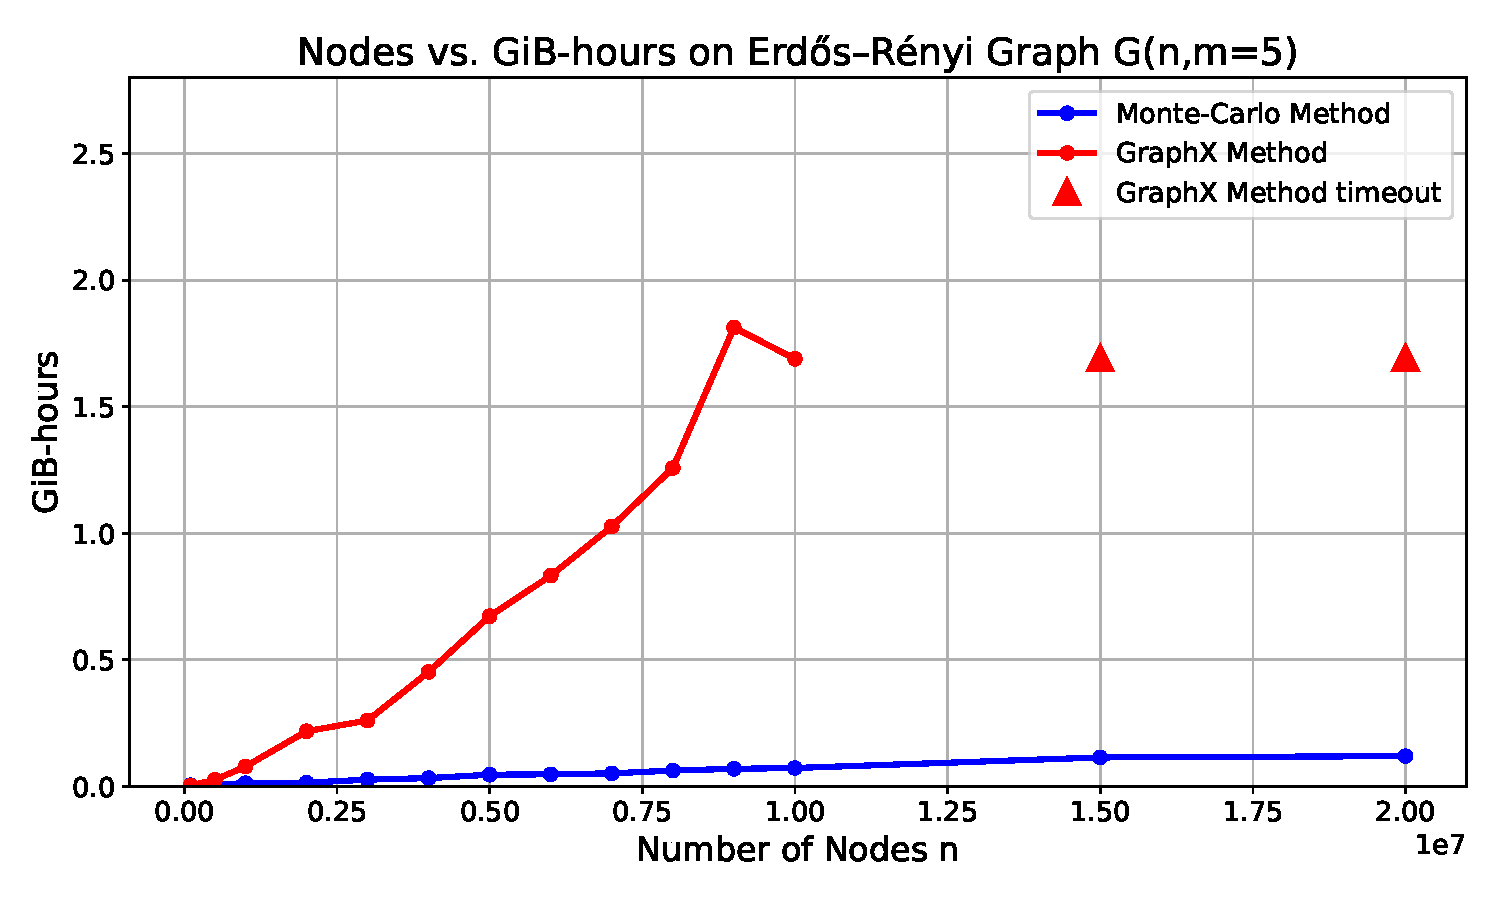
\includegraphics[width=\linewidth]{images/plots/ER_5edg/gbhrs_nodes_er_graph_5edges.pdf}
%         \caption{5 edges per node}
%         \label{fig:5cost}
%     \end{subfigure}
%     \begin{subfigure}[t]{0.47\linewidth}
%         \centering
%         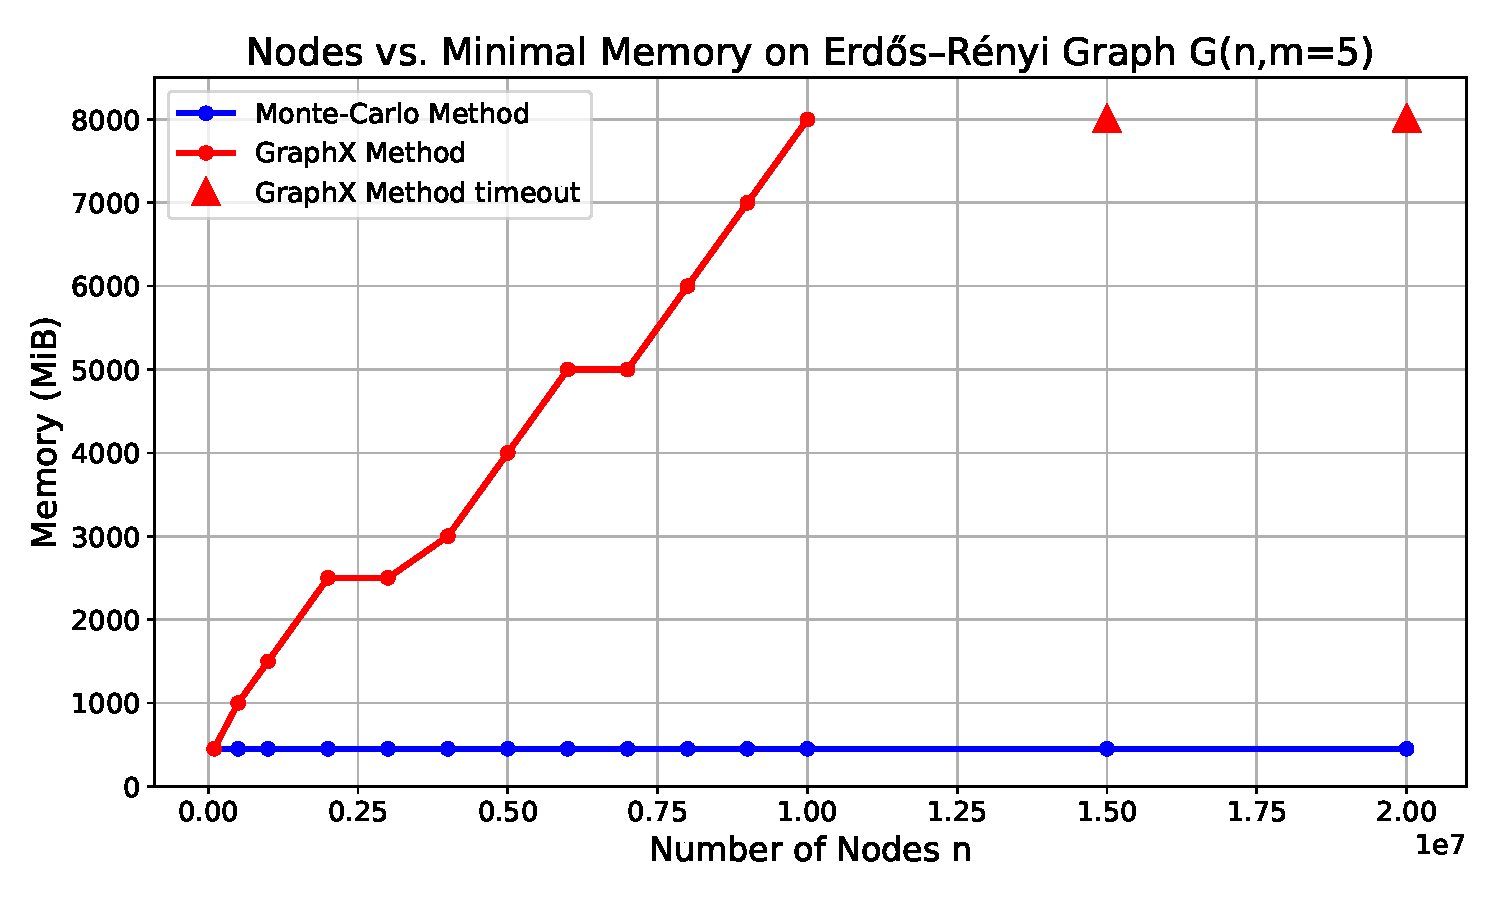
\includegraphics[width=\linewidth]{images/plots/ER_5edg/nodes_vs_mvm_5edges.pdf}
%         \caption{5 edges per node}
%         \label{fig:5mvm}
%     \end{subfigure}
% \end{figure}

%%%%%%% ER Graphs %%%%%%%
Next the plots of the synthetic graphs are analyzed. 


\subsubsection{Performance Plots}
\subsubsection{Accuracy Plots}
\subsubsection{Cost Plots}
\subsubsection{Graph Size vs. Runtime/Memory Plots}
% Include figures/tables: performance vs. accuracy vs. memory.

\subsection{Discussion}
\subsubsection{Trade-offs}
\subsubsection{Experimental setup: realistic?}
\subsubsection{Monte Carlo Approach: good Alternative?}
% Interpret results and explain when your approach is advantageous.

\newpage
\section{Conclusion}
% Summary of your work and suggestions for future research (e.g., better partitioning, dynamic walker allocation).
\newpage
\bibliography{references}

\end{document}
